%%%%%%%%%%%%  Generated using docx2latex.com  %%%%%%%%%%%%%%

%%%%%%%%%%%%  v2.0.0-beta  %%%%%%%%%%%%%%

\documentclass[12pt]{article}
\usepackage{amsmath}
\usepackage{latexsym}
\usepackage{amsfonts}
\usepackage[normalem]{ulem}
\usepackage{soul}
\usepackage{array}
\usepackage{amssymb}
\usepackage{extarrows}
\usepackage{graphicx}
\usepackage[backend=biber,
style=numeric,
sorting=none,
isbn=false,
doi=false,
url=false,
]{biblatex}\addbibresource{bibliography.bib}

\usepackage{subfig}
\usepackage{wrapfig}
\usepackage{wasysym}
\usepackage{enumitem}
\usepackage{adjustbox}
\usepackage{ragged2e}
\usepackage[svgnames,table]{xcolor}
\usepackage{tikz}
\usepackage{longtable}
\usepackage{changepage}
\usepackage{setspace}
\usepackage{hhline}
\usepackage{multicol}
\usepackage{tabto}
\usepackage{float}
\usepackage{multirow}
\usepackage{makecell}
\usepackage{fancyhdr}
\usepackage[toc,page]{appendix}
\usepackage[hidelinks]{hyperref}
\usetikzlibrary{shapes.symbols,shapes.geometric,shadows,arrows.meta}
\tikzset{>={Latex[width=1.5mm,length=2mm]}}
\usepackage{flowchart}\usepackage[paperheight=11.0in,paperwidth=8.5in,left=1.0in,right=1.0in,top=1.0in,bottom=1.0in,headheight=1in]{geometry}
\usepackage[utf8]{inputenc}
\usepackage[T1]{fontenc}
\TabPositions{0.5in,1.0in,1.5in,2.0in,2.5in,3.0in,3.5in,4.0in,4.5in,5.0in,5.5in,6.0in,}

\urlstyle{same}

\renewcommand{\_}{\kern-1.5pt\textunderscore\kern-1.5pt}

 %%%%%%%%%%%%  Set Depths for Sections  %%%%%%%%%%%%%%

% 1) Section
% 1.1) SubSection
% 1.1.1) SubSubSection
% 1.1.1.1) Paragraph
% 1.1.1.1.1) Subparagraph


\setcounter{tocdepth}{5}
\setcounter{secnumdepth}{5}


 %%%%%%%%%%%%  Set Depths for Nested Lists created by \begin{enumerate}  %%%%%%%%%%%%%%


\setlistdepth{9}
\renewlist{enumerate}{enumerate}{9}
		\setlist[enumerate,1]{label=\arabic*)}
		\setlist[enumerate,2]{label=\alph*)}
		\setlist[enumerate,3]{label=(\roman*)}
		\setlist[enumerate,4]{label=(\arabic*)}
		\setlist[enumerate,5]{label=(\Alph*)}
		\setlist[enumerate,6]{label=(\Roman*)}
		\setlist[enumerate,7]{label=\arabic*}
		\setlist[enumerate,8]{label=\alph*}
		\setlist[enumerate,9]{label=\roman*}

\renewlist{itemize}{itemize}{9}
		\setlist[itemize]{label=$\cdot$}
		\setlist[itemize,1]{label=\textbullet}
		\setlist[itemize,2]{label=$\circ$}
		\setlist[itemize,3]{label=$\ast$}
		\setlist[itemize,4]{label=$\dagger$}
		\setlist[itemize,5]{label=$\triangleright$}
		\setlist[itemize,6]{label=$\bigstar$}
		\setlist[itemize,7]{label=$\blacklozenge$}
		\setlist[itemize,8]{label=$\prime$}

\setlength{\topsep}{0pt}\setlength{\parskip}{8.04pt}
\setlength{\parindent}{0pt}

 %%%%%%%%%%%%  This sets linespacing (verticle gap between Lines) Default=1 %%%%%%%%%%%%%%


\renewcommand{\arraystretch}{1.3}


%%%%%%%%%%%%%%%%%%%% Document code starts here %%%%%%%%%%%%%%%%%%%%



\begin{document}
\begin{Center}
{\fontsize{28pt}{33.6pt}\selectfont Exploratory Assignment\par}
\end{Center}\par

\begin{Center}
{\fontsize{14pt}{16.8pt}\selectfont COE17B010\par}
\end{Center}\par

\begin{Center}
{\fontsize{28pt}{33.6pt}\selectfont Q1\par}
\end{Center}\par

{\fontsize{14pt}{16.8pt}\selectfont Understand the working of Hyperlink Induced Topic Search (HITS). Give a pseudocode and illustrate the same over a sample dataset of your choice.\par}\par

{\fontsize{14pt}{16.8pt}\selectfont \uline{Introduction:}\par}\par

\setlength{\parskip}{0.0pt}
\textbf{Hyperlink Induced Topic Search }(HITS) Algorithm is a Link Analysis Algorithm that rates webpages, developed by Jon Kleinberg. This algorithm is used to the web link-structures to discover and rank the webpages relevant for a particular search.\\
HITS uses hubs and authorities to define a recursive relationship between webpages. Before understanding the HITS Algorithm, we first need to know about Hubs and Authorities.\par

\begin{itemize}
	\item Given a query to a Search Engine, the set of highly relevant web pages are called \textbf{Roots}. They are potential \textbf{Authorities}.\par

	\item Pages which are not very relevant but point to pages in the Root are called \textbf{Hubs}. Thus, an Authority is a page that many hubs link to whereas a Hub is a page that links to many authorities.
\end{itemize}\par


\vspace{\baselineskip}
\setlength{\parskip}{8.04pt}
{\fontsize{14pt}{16.8pt}\selectfont \uline{Pseudo Code:}\par}\par

\setlength{\parskip}{0.0pt}
Fix iterations: k\par

\begin{enumerate}
	\item Each node is assigned a Hub score = 1 and an Authority score = 1.\par

	\item Repeat k times:\par

\begin{enumerate}
	\item \textbf{Hub update:} \par

 \[ Each node’s Hub score =  \sum _{}^{} \left( Authority score of each node it points to \right)   \] \par

	\item \textbf{Authority update:} \par

 \[ Each node’s Authority score =  \sum _{}^{} \left( Hub score of each node pointing to it \right)   \] \par

	\item Normalize the scores by dividing each Hub score by square root of the sum of the squares of all Hub scores, and dividing each Authority score by square root of the sum of the squares of all Authority scores. (optional)
\end{enumerate}
\end{enumerate}\par


\vspace{\baselineskip}
\setlength{\parskip}{8.04pt}

\vspace{\baselineskip}

\vspace{\baselineskip}

\vspace{\baselineskip}
{\fontsize{14pt}{16.8pt}\selectfont \uline{Trace:}\par}\par

Input Dataset\par



%%%%%%%%%%%%%%%%%%%% Figure/Image No: 1 starts here %%%%%%%%%%%%%%%%%%%%

\begin{figure}[H]
	\begin{Center}
		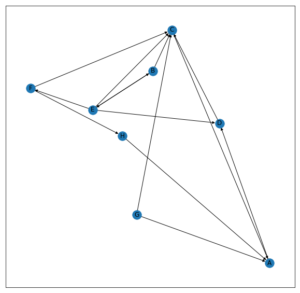
\includegraphics[width=3.12in,height=1.82in]{./media/image1.png}
	\end{Center}
\end{figure}


%%%%%%%%%%%%%%%%%%%% Figure/Image No: 1 Ends here %%%%%%%%%%%%%%%%%%%%

\par

Fixing k = 3, \par

\setlength{\parskip}{7.44pt}
Initially,\par

Hub\ Scores:\ \ \ \ \ \   Authority Scores:\par

A\ ->\ 1\ \ \ \ \ \ \ \ \ \    A -> 1\par

B\ ->\ 1\ \ \ \ \ \ \ \ \ \    B -> 1\par

C\ ->\ 1\ \ \ \ \ \ \ \ \ \    C -> 1\par

D\ ->\ 1\ \ \ \ \ \ \ \ \ \    D -> 1\par

E\ ->\ 1\ \ \ \ \ \ \ \ \ \    E -> 1\par

F\ ->\ 1\ \ \ \ \ \ \ \ \ \    F -> 1\par

G\ ->\ 1\ \ \ \ \ \ \ \ \ \    G -> 1\par

H\ ->\ 1\ \ \ \ \ \ \ \ \ \    H -> 1\par


\vspace{\baselineskip}After 1st iteration,\par

Hub\ Scores:\ \ \ \ \ \   Authority Scores:\par

A\ ->\ 1\ \ \ \ \ \ \ \ \ \    A -> 3\par

B\ ->\ 2\ \ \ \ \ \ \ \ \ \    B -> 2\par

C\ ->\ 1\ \ \ \ \ \ \ \ \ \    C -> 4\par

D\ ->\ 2\ \ \ \ \ \ \ \ \ \    D -> 2\par

E\ ->\ 4\ \ \ \ \ \ \ \ \ \    E -> 1\par

F\ ->\ 1\ \ \ \ \ \ \ \ \ \    F -> 1\par

G\ ->\ 2\ \ \ \ \ \ \ \ \ \    G -> 0\par

H\ ->\ 1\ \ \ \ \ \ \ \ \ \    H -> 1\par


\vspace{\baselineskip}After 2nd iteration,\par

Hub\ Scores:\ \ \ \ \ \   Authority Scores:\par

A\ ->\ 2\ \ \ \ \ \ \ \ \ \    A -> 4\par

B\ ->\ 5\ \ \ \ \ \ \ \ \ \    B -> 6\par

C\ ->\ 3\ \ \ \ \ \ \ \ \ \    C -> 7\par

D\ ->\ 6\ \ \ \ \ \ \ \ \ \    D -> 5\par

E\ ->\ 9\ \ \ \ \ \ \ \ \ \    E -> 2\par

F\ ->\ 1\ \ \ \ \ \ \ \ \ \    F -> 4\par

G\ ->\ 7\ \ \ \ \ \ \ \ \ \    G -> 0\par

H\ ->\ 3\ \ \ \ \ \ \ \ \ \    H -> 1\par


\vspace{\baselineskip}After 3rd iteration,\par

Hub\ Scores:\ \ \ \ \ \   Authority Scores:\par

A\ ->\ 5\ \ \ \ \ \ \ \ \ \    A -> 13\par

B\ ->\ 9\ \ \ \ \ \ \ \ \ \    B -> 15\par

C\ ->\ 4\ \ \ \ \ \ \ \ \ \    C -> 27\par

D\ ->\ 13\ \ \ \ \ \ \ \ \    D -> 11\par

E\ ->\ 22\ \ \ \ \ \ \ \ \    E -> 5\par

F\ ->\ 1\ \ \ \ \ \ \ \ \ \    F -> 9\par

G\ ->\ 11\ \ \ \ \ \ \ \ \    G -> 0\par

H\ ->\ 4\ \ \ \ \ \ \ \ \ \    H -> 3\par


\vspace{\baselineskip}
\vspace{\baselineskip}
\vspace{\baselineskip}
\setlength{\parskip}{8.04pt}

\vspace{\baselineskip}

\vspace{\baselineskip}

\vspace{\baselineskip}

\vspace{\baselineskip}

\vspace{\baselineskip}
\begin{Center}
{\fontsize{28pt}{33.6pt}\selectfont Q2\par}
\end{Center}\par

{\fontsize{14pt}{16.8pt}\selectfont Understand the working of BIRCH and DBSCAN clustering algorithms. Give a pseudocode and trace the same over a sample dataset of your choice.\par}\par

\begin{enumerate}
	\item {\fontsize{20pt}{24.0pt}\selectfont BIRCH Clustering\par}\par

{\fontsize{14pt}{16.8pt}\selectfont \uline{Introduction:}\par}\par

Balanced Iterative Reducing and Clustering using Hierarchies, or BIRCH for short, deals with large datasets by first generating a more compact summary that retains as much distribution information as possible, and then clustering the data summary instead of the original dataset. BIRCH actually complements other clustering algorithms by virtue if the fact that different clustering algorithms can be applied to the summary produced by BIRCH. BIRCH can only deal with metric attributes (similar to the kind of features KMEANS can handle). A metric attribute is one whose values can be represented by explicit coordinates in an Euclidean space (no categorical variables).\par

{\fontsize{14pt}{16.8pt}\selectfont \uline{Pseudo Code:}\par}\par

Take the initial Data, \par

\setlength{\parskip}{7.44pt}
\begin{itemize}
	\item {\fontsize{11pt}{13.2pt}\selectfont \textbf{\textcolor[HTML]{333333}{Phase 1:}}\textcolor[HTML]{333333}{ Load data into memory}\par}\par

{\fontsize{11pt}{13.2pt}\selectfont \textcolor[HTML]{333333}{Scan DB and load data into memory by building a CF tree. If memory is exhausted rebuild the tree from the leaf node.}\par}\par

	\item {\fontsize{11pt}{13.2pt}\selectfont \textbf{\textcolor[HTML]{333333}{Phase 2:}}\textcolor[HTML]{333333}{ Condense data}\par}\par

{\fontsize{11pt}{13.2pt}\selectfont \textcolor[HTML]{333333}{Resize the data set by building a smaller CF tree}\par}\par

{\fontsize{11pt}{13.2pt}\selectfont \textcolor[HTML]{333333}{Remove more outliers}\par}\par

{\fontsize{11pt}{13.2pt}\selectfont \textcolor[HTML]{333333}{Condensing is optional}\par}\par

	\item {\fontsize{11pt}{13.2pt}\selectfont \textbf{\textcolor[HTML]{333333}{Phase 3:}}\textcolor[HTML]{333333}{ Global clustering}\par}\par

{\fontsize{11pt}{13.2pt}\selectfont \textcolor[HTML]{333333}{Use existing clustering algorithm (e.g. KMEANS, HC) on CF entries}\par}\par

	\item {\fontsize{11pt}{13.2pt}\selectfont \textbf{\textcolor[HTML]{333333}{Phase 4:}}\textcolor[HTML]{333333}{ Cluster refining}\par}
\end{itemize}\par

\begin{adjustwidth}{0.5in}{0.0in}
{\fontsize{11pt}{13.2pt}\selectfont \textcolor[HTML]{333333}{Refining is optional}\par}\par

\end{adjustwidth}

\begin{adjustwidth}{0.5in}{0.0in}
{\fontsize{11pt}{13.2pt}\selectfont \textcolor[HTML]{333333}{Fixes the problem with CF trees where same valued data points may be assigned to different leaf entries.}\par}\par

\end{adjustwidth}

{\fontsize{14pt}{16.8pt}\selectfont \uline{Trace:}\par}\par

{\fontsize{11pt}{13.2pt}\selectfont \textcolor[HTML]{333333}{CF= (N, LS, SS)}\par}\par

 \[ N=No of data points \] \par

 \[ LS=  \sum _{i=1}^{N}X_{i} \] \par

 \[ SS= \sum _{i=1}^{N}X_{i}^{2} \] \par

Example Trace\par



%%%%%%%%%%%%%%%%%%%% Figure/Image No: 2 starts here %%%%%%%%%%%%%%%%%%%%

\begin{figure}[H]
	\begin{Center}
		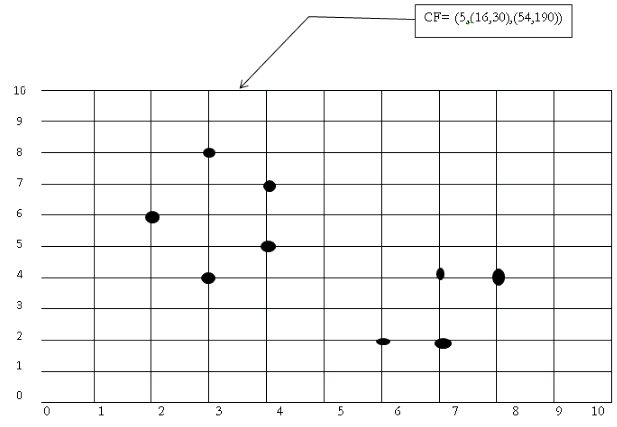
\includegraphics[width=6.42in,height=4.45in]{./media/image2.png}
	\end{Center}
\end{figure}


%%%%%%%%%%%%%%%%%%%% Figure/Image No: 2 Ends here %%%%%%%%%%%%%%%%%%%%

\par

{\fontsize{11pt}{13.2pt}\selectfont \textcolor[HTML]{333333}{(3,4) (2,6)(4,5)(4,7)(3,8)}\par}\par

{\fontsize{11pt}{13.2pt}\selectfont \textcolor[HTML]{333333}{N=5}\par}\par

{\fontsize{11pt}{13.2pt}\selectfont \textcolor[HTML]{333333}{NS= (16, 30 ) i.e. 3+2+4+4+3=16 and 4+6+5+7+8=30}\par}\par

\setlength{\parskip}{0.0pt}
{\fontsize{11pt}{13.2pt}\selectfont \textcolor[HTML]{333333}{SS=(54,190)=3\textsuperscript{2}+2\textsuperscript{2}+4\textsuperscript{2}+4\textsuperscript{2}+3\textsuperscript{2}=54  and  42+62+52+72+82= 190}\par}\par


\vspace{\baselineskip}

\vspace{\baselineskip}

\vspace{\baselineskip}

\vspace{\baselineskip}

\vspace{\baselineskip}

\vspace{\baselineskip}
Input Data\par



%%%%%%%%%%%%%%%%%%%% Figure/Image No: 3 starts here %%%%%%%%%%%%%%%%%%%%

\begin{figure}[H]
	\begin{Center}
		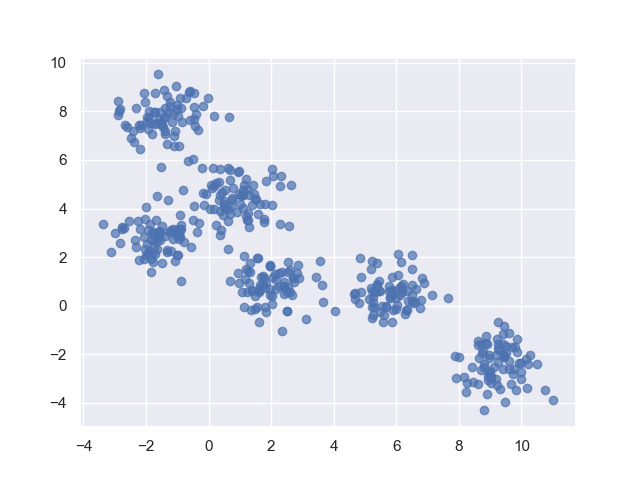
\includegraphics[width=4.85in,height=2.82in]{./media/image3.png}
	\end{Center}
\end{figure}


%%%%%%%%%%%%%%%%%%%% Figure/Image No: 3 Ends here %%%%%%%%%%%%%%%%%%%%

\par

After Clustering, \par



%%%%%%%%%%%%%%%%%%%% Figure/Image No: 4 starts here %%%%%%%%%%%%%%%%%%%%

\begin{figure}[H]
	\begin{Center}
		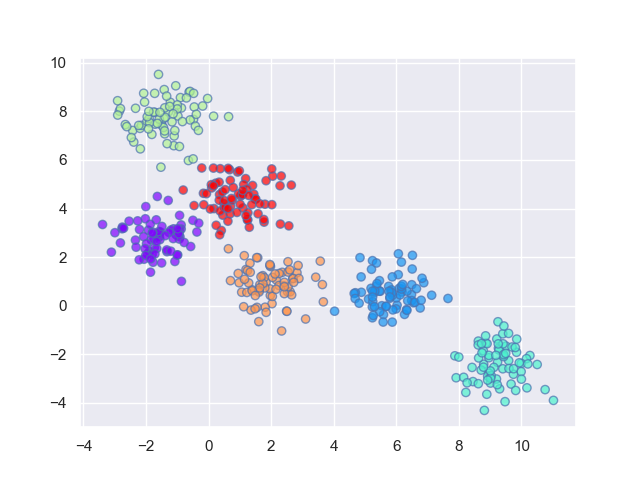
\includegraphics[width=6.4in,height=4.8in]{./media/image4.png}
	\end{Center}
\end{figure}


%%%%%%%%%%%%%%%%%%%% Figure/Image No: 4 Ends here %%%%%%%%%%%%%%%%%%%%

\par


\vspace{\baselineskip}

\vspace{\baselineskip}

\vspace{\baselineskip}
\setlength{\parskip}{8.04pt}
	\item {\fontsize{20pt}{24.0pt}\selectfont DBSCAN Clustering\par}
\end{enumerate}\par

{\fontsize{14pt}{16.8pt}\selectfont \uline{Introduction:}\par}\par

\setlength{\parskip}{0.0pt}
Fundamentally, all clustering methods use the same approach i.e. first we calculate similarities and then we use it to cluster the data points into groups or batches. Here we will focus on \textbf{Density-based spatial clustering of applications with noise} (DBSCAN) clustering method.\par

Clusters are dense regions in the data space, separated by regions of the lower density of points. The \textbf{\textit{DBSCAN algorithm}} is based on this intuitive notion of $``$clusters$"$  and $``$noise$"$ . The key idea is that for each point of a cluster, the neighborhood of a given radius has to contain at least a minimum number of points.\par

\textbf{DBSCAN algorithm requires two parameters –}\par

\begin{enumerate}[label*=\arabic*.]
	\item \textbf{eps} : It defines the neighborhood around a data point i.e. if the distance between two points is lower or equal to ‘eps’ then they are considered as neighbors. If the eps value is chosen too small then large part of the data will be considered as outliers. If it is chosen very large then the clusters will merge and majority of the data points will be in the same clusters. One way to find the eps value is based on the \textbf{\textit{k-distance graph}}.\par

	\item \textbf{MinPts}: Minimum number of neighbors (data points) within eps radius. Larger the dataset, the larger value of MinPts must be chosen. As a general rule, the minimum MinPts can be derived from the number of dimensions D in the dataset as, MinPts >= D+1. The minimum value of MinPts must be chosen at least 3.\\

\end{enumerate}\par

\begin{adjustwidth}{0.38in}{0.0in}
\textbf{\textit{In this algorithm, we have 3 types of data points.}}\par

\end{adjustwidth}

\begin{adjustwidth}{0.38in}{0.0in}
\textbf{\textit{Core Point}}\textit{: A point is a core point if it has more than MinPts points within eps.\\
\textbf{Border Point}: A point which has fewer than MinPts within eps but it is in the neighborhood of a core point.\\
\textbf{Noise or outlier}: A point which is not a core point or border point.}\par

\end{adjustwidth}

{\fontsize{14pt}{16.8pt}\selectfont \uline{Pseudo Code:}\par}\par

\begin{enumerate}[label*=\arabic*.]
	\item Find all the neighbor points within eps and identify the core points or visited with more than MinPts neighbors.\par

	\item For each core point if it is not already assigned to a cluster, create a new cluster.\par

	\item Find recursively all its density connected points and assign them to the same cluster as the core point.\\
A point\textit{ a} and \textit{b} are said to be density connected if there exist a point \textit{c} which has a sufficient number of points in its neighbors and both the points\textit{ a} and \textit{b} are within the \textit{eps distance}. This is a chaining process. So, if \textit{b} is neighbor of \textit{c}, \textit{c} is neighbor of\textit{ d}, \textit{d} is neighbor of \textit{e}, which in turn is neighbor of \textit{a} implies that \textit{b} is neighbor of\textit{ a}.\par

	\item Iterate through the remaining unvisited points in the dataset. Those points that do not belong to any cluster are noise.
\end{enumerate}\par


\vspace{\baselineskip}

\vspace{\baselineskip}

\vspace{\baselineskip}
{\fontsize{14pt}{16.8pt}\selectfont \uline{Trace:}\par}\par



%%%%%%%%%%%%%%%%%%%% Figure/Image No: 5 starts here %%%%%%%%%%%%%%%%%%%%

\begin{figure}[H]
	\begin{Center}
		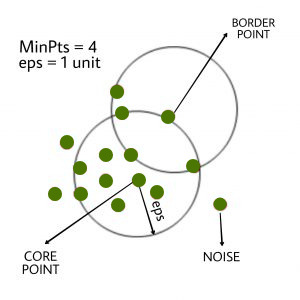
\includegraphics[width=3.12in,height=3.12in]{./media/image5.jpeg}
	\end{Center}
\end{figure}


%%%%%%%%%%%%%%%%%%%% Figure/Image No: 5 Ends here %%%%%%%%%%%%%%%%%%%%

\par

Here, first we identify core points and as shown in diagram, \par

The marked point is a core point as it has > 4 neighbors within eps 1 unit.\par

Hence the core point is assigned a cluster A.\par

Similarly, we can identify that all the points are belonging to cluster A itself as neighbors of the central core point also have > 4 neighbors within 1-unit eps thereby connecting their neighbors under same cluster as them, i.e. Cluster A.\par

Only that 1 point is marked noise as it has no nearby points with > 4 neighbors within 1-unit eps. Hence it does not belong to any cluster, hence noise.\par

Input Data\par



%%%%%%%%%%%%%%%%%%%% Figure/Image No: 6 starts here %%%%%%%%%%%%%%%%%%%%

\begin{figure}[H]
	\begin{Center}
		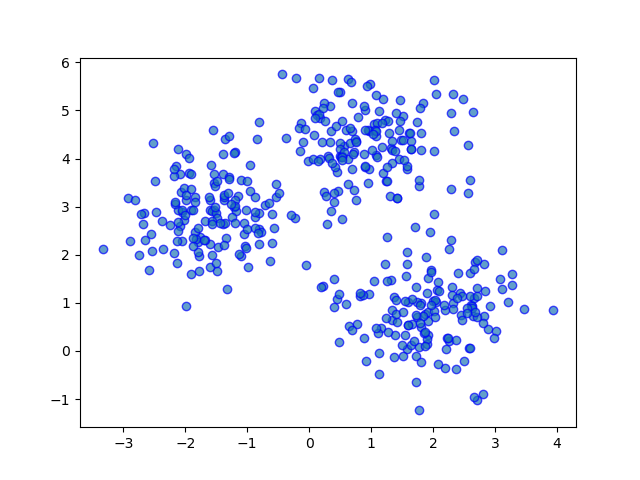
\includegraphics[width=3.37in,height=2.52in]{./media/image6.png}
	\end{Center}
\end{figure}


%%%%%%%%%%%%%%%%%%%% Figure/Image No: 6 Ends here %%%%%%%%%%%%%%%%%%%%

\par


\vspace{\baselineskip}

\vspace{\baselineskip}
Output Clusters\par



%%%%%%%%%%%%%%%%%%%% Figure/Image No: 7 starts here %%%%%%%%%%%%%%%%%%%%

\begin{figure}[H]
	\begin{Center}
		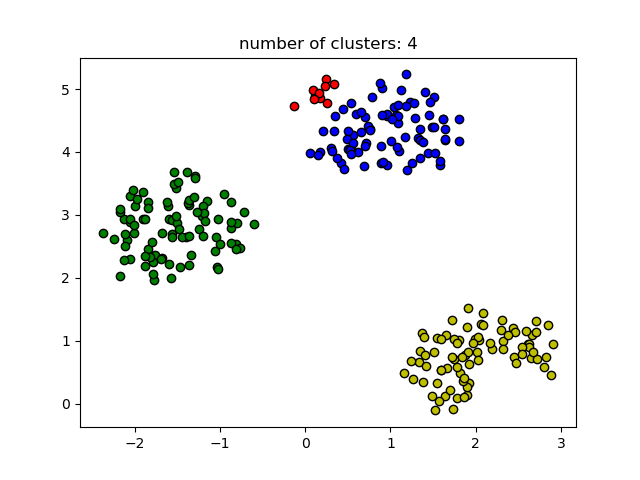
\includegraphics[width=4.83in,height=3.62in]{./media/image7.png}
	\end{Center}
\end{figure}


%%%%%%%%%%%%%%%%%%%% Figure/Image No: 7 Ends here %%%%%%%%%%%%%%%%%%%%

\par


\vspace{\baselineskip}
\setlength{\parskip}{8.04pt}

\vspace{\baselineskip}

\vspace{\baselineskip}

\vspace{\baselineskip}

\vspace{\baselineskip}

\vspace{\baselineskip}

\vspace{\baselineskip}

\vspace{\baselineskip}

\vspace{\baselineskip}

\vspace{\baselineskip}

\vspace{\baselineskip}

\vspace{\baselineskip}
\begin{Center}
{\fontsize{28pt}{33.6pt}\selectfont Q3\par}
\end{Center}\par

{\fontsize{14pt}{16.8pt}\selectfont Understand the different types of selection, cross-over, mutation operation that are employed by Genetic algorithms. Illustrate the working of each over a population of chromosomes (Refer David Goldberg or any other online sources). Explore a minimum of at least 4 to 5 operators under each type.\par}\par

\begin{enumerate}
	\item {\fontsize{20pt}{24.0pt}\selectfont Selection Operators\par}\par

{\fontsize{14pt}{16.8pt}\selectfont \uline{Roulette Wheel Selection}\par}\par

\setlength{\parskip}{7.2pt}
\begin{justify}
In a roulette wheel selection, the circular wheel is divided as described before. A fixed point is chosen on the wheel circumference as shown and the wheel is rotated. The region of the wheel which comes in front of the fixed point is chosen as the parent. For the second parent, the same process is repeated.
\end{justify}\par



%%%%%%%%%%%%%%%%%%%% Figure/Image No: 8 starts here %%%%%%%%%%%%%%%%%%%%

\begin{figure}[H]
	\begin{Center}
		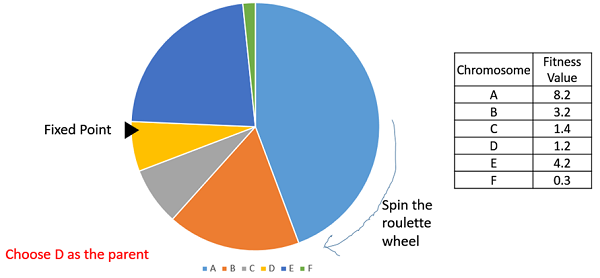
\includegraphics[width=6.25in,height=2.9in]{./media/image8.png}
	\end{Center}
\end{figure}


%%%%%%%%%%%%%%%%%%%% Figure/Image No: 8 Ends here %%%%%%%%%%%%%%%%%%%%

\setlength{\parskip}{0.0pt}
\par

\setlength{\parskip}{7.2pt}
\begin{justify}
It is clear that a fitter individual has a greater pie on the wheel and therefore a greater chance of landing in front of the fixed point when the wheel is rotated. Therefore, the probability of choosing an individual depends directly on its fitness.
\end{justify}\par

\begin{justify}
Implementation wise, we use the following steps $-$ 
\end{justify}\par

\begin{itemize}
	\item Calculate S = the sum of a fitnesses.\par

	\item Generate a random number between 0 and S.\par

	\item Starting from the top of the population, keep adding the finesses to the partial sum P, till P<S.\par

	\item The individual for which P exceeds S is the chosen individual.
\end{itemize}\par


\vspace{\baselineskip}

\vspace{\baselineskip}
\begin{adjustwidth}{0.0in}{0.03in}
\begin{justify}
{\fontsize{14pt}{16.8pt}\selectfont \uline{Stochastic Universal Sampling (SUS)}\par}
\end{justify}\par

\end{adjustwidth}


\vspace{\baselineskip}
\begin{adjustwidth}{0.03in}{0.03in}
\begin{justify}
Stochastic Universal Sampling is quite similar to Roulette wheel selection, however instead of having just one fixed point, we have multiple fixed points as shown in the following image. Therefore, all the parents are chosen in just one spin of the wheel. Also, such a setup encourages the highly fit individuals to be chosen at least once.
\end{justify}\par

\end{adjustwidth}



%%%%%%%%%%%%%%%%%%%% Figure/Image No: 9 starts here %%%%%%%%%%%%%%%%%%%%

\begin{figure}[H]
	\begin{Center}
		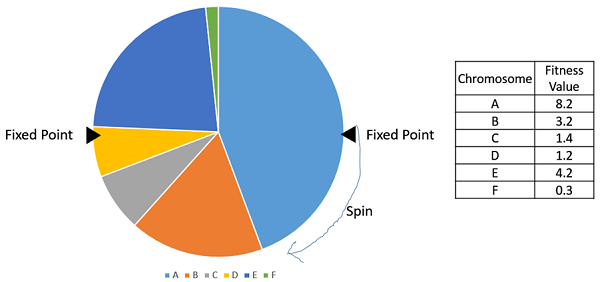
\includegraphics[width=6.25in,height=2.93in]{./media/image9.png}
	\end{Center}
\end{figure}


%%%%%%%%%%%%%%%%%%%% Figure/Image No: 9 Ends here %%%%%%%%%%%%%%%%%%%%

\setlength{\parskip}{0.0pt}
\par

\setlength{\parskip}{7.2pt}
\begin{adjustwidth}{0.03in}{0.03in}
\begin{justify}
It is to be noted that fitness proportionate selection methods don’t work for cases where the fitness can take a negative value.
\end{justify}\par

\end{adjustwidth}


\vspace{\baselineskip}
\begin{adjustwidth}{0.03in}{0.03in}
\begin{justify}
{\fontsize{14pt}{16.8pt}\selectfont \uline{Tournament Selection}\par}
\end{justify}\par

\end{adjustwidth}

\begin{adjustwidth}{0.03in}{0.03in}
{\fontsize{11pt}{13.2pt}\selectfont In K-Way tournament selection, we select K individuals from the population at random and select the best out of these to become a parent. The same process is repeated for selecting the next parent. Tournament Selection is also extremely popular in literature as it can even work with negative fitness values.\par}\par

\end{adjustwidth}



%%%%%%%%%%%%%%%%%%%% Figure/Image No: 10 starts here %%%%%%%%%%%%%%%%%%%%

\begin{figure}[H]
	\begin{Center}
		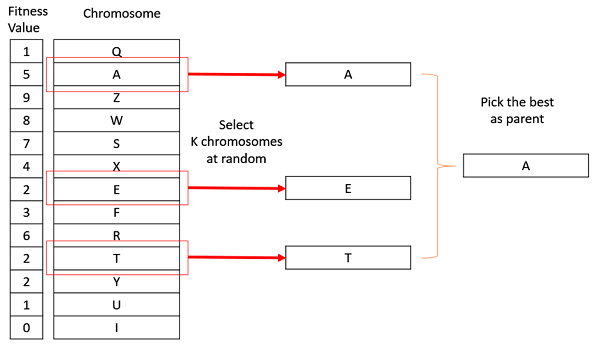
\includegraphics[width=6.24in,height=2.51in]{./media/image10.png}
	\end{Center}
\end{figure}


%%%%%%%%%%%%%%%%%%%% Figure/Image No: 10 Ends here %%%%%%%%%%%%%%%%%%%%

\setlength{\parskip}{8.04pt}
\par

{\fontsize{14pt}{16.8pt}\selectfont \uline{Rank Selection}\par}\par

\setlength{\parskip}{7.2pt}
\begin{adjustwidth}{0.03in}{0.03in}
{\fontsize{11pt}{13.2pt}\selectfont Rank Selection also works with negative fitness values and is mostly used when the individuals in the population have very close fitness values (this happens usually at the end of the run). This leads to each individual having an almost equal share of the pie (like in case of fitness proportionate selection) as shown in the following image and hence each individual no matter how fit relative to each other has an approximately same probability of getting selected as a parent. This in turn leads to a loss in the selection pressure towards fitter individuals, making the GA to make poor parent selections in such situations.\par}\par

\end{adjustwidth}



%%%%%%%%%%%%%%%%%%%% Figure/Image No: 11 starts here %%%%%%%%%%%%%%%%%%%%

\begin{figure}[H]
	\begin{Center}
		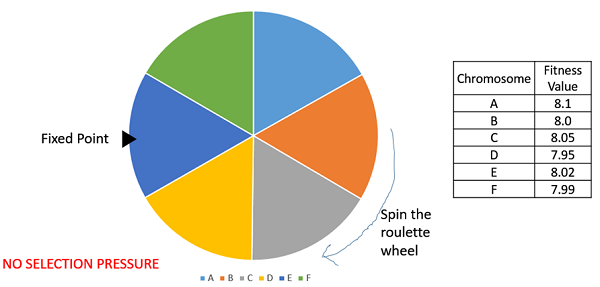
\includegraphics[width=6.24in,height=2.44in]{./media/image11.png}
	\end{Center}
\end{figure}


%%%%%%%%%%%%%%%%%%%% Figure/Image No: 11 Ends here %%%%%%%%%%%%%%%%%%%%

\setlength{\parskip}{8.04pt}
\par

\setlength{\parskip}{7.2pt}
\begin{adjustwidth}{0.03in}{0.03in}
{\fontsize{11pt}{13.2pt}\selectfont In this, we remove the concept of a fitness value while selecting a parent. However, every individual in the population is ranked according to their fitness. The selection of the parents depends on the rank of each individual and not the fitness. The higher ranked individuals are preferred more than the lower ranked ones.\par}\par

\end{adjustwidth}



%%%%%%%%%%%%%%%%%%%% Table No: 1 starts here %%%%%%%%%%%%%%%%%%%%


\begin{table}[H]
 			\centering
\begin{tabular}{p{2.67in}p{2.63in}p{1.19in}}
\hline
%row no:1
\multicolumn{1}{|p{2.67in}}{\cellcolor[HTML]{EEEEEE}\Centering {\fontsize{10pt}{12.0pt}\selectfont \textbf{Chromosome}}} & 
\multicolumn{1}{|p{2.63in}}{\cellcolor[HTML]{EEEEEE}\Centering {\fontsize{10pt}{12.0pt}\selectfont \textbf{Fitness Value}}} & 
\multicolumn{1}{|p{1.19in}|}{\cellcolor[HTML]{EEEEEE}\Centering {\fontsize{10pt}{12.0pt}\selectfont \textbf{Rank}}} \\
\hhline{---}
%row no:2
\multicolumn{1}{|p{2.67in}}{\Centering {\fontsize{10pt}{12.0pt}\selectfont A}} & 
\multicolumn{1}{|p{2.63in}}{\Centering {\fontsize{10pt}{12.0pt}\selectfont 8.1}} & 
\multicolumn{1}{|p{1.19in}|}{\Centering {\fontsize{10pt}{12.0pt}\selectfont 1}} \\
\hhline{---}
%row no:3
\multicolumn{1}{|p{2.67in}}{\Centering {\fontsize{10pt}{12.0pt}\selectfont B}} & 
\multicolumn{1}{|p{2.63in}}{\Centering {\fontsize{10pt}{12.0pt}\selectfont 8.0}} & 
\multicolumn{1}{|p{1.19in}|}{\Centering {\fontsize{10pt}{12.0pt}\selectfont 4}} \\
\hhline{---}
%row no:4
\multicolumn{1}{|p{2.67in}}{\Centering {\fontsize{10pt}{12.0pt}\selectfont C}} & 
\multicolumn{1}{|p{2.63in}}{\Centering {\fontsize{10pt}{12.0pt}\selectfont 8.05}} & 
\multicolumn{1}{|p{1.19in}|}{\Centering {\fontsize{10pt}{12.0pt}\selectfont 2}} \\
\hhline{---}
%row no:5
\multicolumn{1}{|p{2.67in}}{\Centering {\fontsize{10pt}{12.0pt}\selectfont D}} & 
\multicolumn{1}{|p{2.63in}}{\Centering {\fontsize{10pt}{12.0pt}\selectfont 7.95}} & 
\multicolumn{1}{|p{1.19in}|}{\Centering {\fontsize{10pt}{12.0pt}\selectfont 6}} \\
\hhline{---}
%row no:6
\multicolumn{1}{|p{2.67in}}{\Centering {\fontsize{10pt}{12.0pt}\selectfont E}} & 
\multicolumn{1}{|p{2.63in}}{\Centering {\fontsize{10pt}{12.0pt}\selectfont 8.02}} & 
\multicolumn{1}{|p{1.19in}|}{\Centering {\fontsize{10pt}{12.0pt}\selectfont 3}} \\
\hhline{---}
%row no:7
\multicolumn{1}{|p{2.67in}}{\Centering {\fontsize{10pt}{12.0pt}\selectfont F}} & 
\multicolumn{1}{|p{2.63in}}{\Centering {\fontsize{10pt}{12.0pt}\selectfont 7.99}} & 
\multicolumn{1}{|p{1.19in}|}{\Centering {\fontsize{10pt}{12.0pt}\selectfont 5}} \\
\hhline{---}

\end{tabular}
 \end{table}


%%%%%%%%%%%%%%%%%%%% Table No: 1 ends here %%%%%%%%%%%%%%%%%%%%

\setlength{\parskip}{8.04pt}
{\fontsize{14pt}{16.8pt}\selectfont \uline{Random Selection}\par}\par

\setlength{\parskip}{7.2pt}
\begin{adjustwidth}{0.03in}{0.03in}
{\fontsize{11pt}{13.2pt}\selectfont In this strategy we randomly select parents from the existing population. There is no selection pressure towards fitter individuals and therefore this strategy is usually avoided.\par}\par

\end{adjustwidth}


\vspace{\baselineskip}
\setlength{\parskip}{8.04pt}
	\item {\fontsize{20pt}{24.0pt}\selectfont Crossover Operators\par}\par


\vspace{\baselineskip}
\setlength{\parskip}{7.2pt}
\begin{justify}
{\fontsize{14pt}{16.8pt}\selectfont \uline{One Point Crossover}\par}
\end{justify}\par

\begin{justify}
In this one-point crossover, a random crossover point is selected and the tails of its two parents are swapped to get new off-springs.
\end{justify}\par



%%%%%%%%%%%%%%%%%%%% Figure/Image No: 12 starts here %%%%%%%%%%%%%%%%%%%%

\begin{figure}[H]
	\begin{Center}
		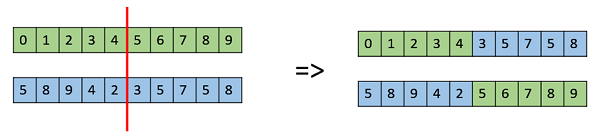
\includegraphics[width=6.25in,height=1.43in]{./media/image12.png}
	\end{Center}
\end{figure}


%%%%%%%%%%%%%%%%%%%% Figure/Image No: 12 Ends here %%%%%%%%%%%%%%%%%%%%

\setlength{\parskip}{0.0pt}
\par

\setlength{\parskip}{7.2pt}
\begin{justify}
{\fontsize{14pt}{16.8pt}\selectfont \uline{Multi Point Crossover}\par}
\end{justify}\par

\begin{justify}
Multi point crossover is a generalization of the one-point crossover wherein alternating segments are swapped to get new off-springs.
\end{justify}\par



%%%%%%%%%%%%%%%%%%%% Figure/Image No: 13 starts here %%%%%%%%%%%%%%%%%%%%

\begin{figure}[H]
	\begin{Center}
		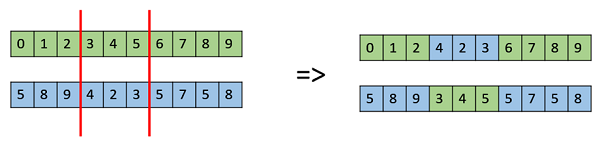
\includegraphics[width=6.25in,height=1.49in]{./media/image13.png}
	\end{Center}
\end{figure}


%%%%%%%%%%%%%%%%%%%% Figure/Image No: 13 Ends here %%%%%%%%%%%%%%%%%%%%

\setlength{\parskip}{0.0pt}
\par

\setlength{\parskip}{7.2pt}
\begin{justify}
{\fontsize{14pt}{16.8pt}\selectfont \uline{Uniform Crossover}\par}
\end{justify}\par

\begin{justify}
In a uniform crossover, we don’t divide the chromosome into segments, rather we treat each gene separately. In this, we essentially flip a coin for each chromosome to decide whether or not it’ll be included in the off-spring. We can also bias the coin to one parent, to have more genetic material in the child from that parent.
\end{justify}\par



%%%%%%%%%%%%%%%%%%%% Figure/Image No: 14 starts here %%%%%%%%%%%%%%%%%%%%

\begin{figure}[H]
	\begin{Center}
		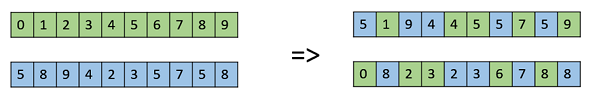
\includegraphics[width=6.25in,height=1.03in]{./media/image14.png}
	\end{Center}
\end{figure}


%%%%%%%%%%%%%%%%%%%% Figure/Image No: 14 Ends here %%%%%%%%%%%%%%%%%%%%

\setlength{\parskip}{0.0pt}
\par

\setlength{\parskip}{7.2pt}
\begin{justify}
{\fontsize{14pt}{16.8pt}\selectfont \uline{Whole Arithmetic Recombination}\par}
\end{justify}\par

\begin{justify}
This is commonly used for integer representations and works by taking the weighted average of the two parents by using the following formulas, 
\end{justify}\par

\setlength{\parskip}{3.72pt}
\begin{itemize}
	\item  \( Child1 =  \alpha .x_{1} +  \left( 1- \alpha  \right) .x_{2} \) \par

	\item  \( Child2 =  \alpha .x_{2} +  \left( 1- \alpha  \right) .x_{1} \) 
\end{itemize}\par

\setlength{\parskip}{7.2pt}
\begin{adjustwidth}{0.03in}{0.03in}
\begin{justify}
Obviously, if  \(  \alpha  = 0.5 \) , then both the children will be identical as shown in the following image.
\end{justify}\par

\end{adjustwidth}



%%%%%%%%%%%%%%%%%%%% Figure/Image No: 15 starts here %%%%%%%%%%%%%%%%%%%%

\begin{figure}[H]
	\begin{Center}
		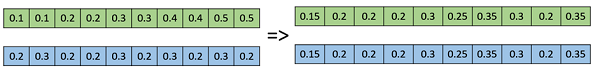
\includegraphics[width=6.25in,height=0.76in]{./media/image15.png}
	\end{Center}
\end{figure}


%%%%%%%%%%%%%%%%%%%% Figure/Image No: 15 Ends here %%%%%%%%%%%%%%%%%%%%

\setlength{\parskip}{0.0pt}
\par


\vspace{\baselineskip}
\setlength{\parskip}{7.2pt}
\begin{adjustwidth}{0.03in}{0.03in}
\begin{justify}
{\fontsize{14pt}{16.8pt}\selectfont \uline{Davis’s Order Crossover (OX1)}\par}
\end{justify}\par

\end{adjustwidth}

\begin{adjustwidth}{0.03in}{0.03in}
\begin{justify}
OX1 is used for permutation-based crossovers with the intention of transmitting information about relative ordering to the off-springs. It works as follows $-$ 
\end{justify}\par

\end{adjustwidth}

\begin{itemize}
	\item Create two random crossover points in the parent and copy the segment between them from the first parent to the first offspring.\par

	\item Now, starting from the second crossover point in the second parent, copy the remaining unused numbers from the second parent to the first child, wrapping around the list.\par

	\item Repeat for the second child with the parent’s role reversed.
\end{itemize}\par



%%%%%%%%%%%%%%%%%%%% Figure/Image No: 16 starts here %%%%%%%%%%%%%%%%%%%%

\begin{figure}[H]
	\begin{Center}
		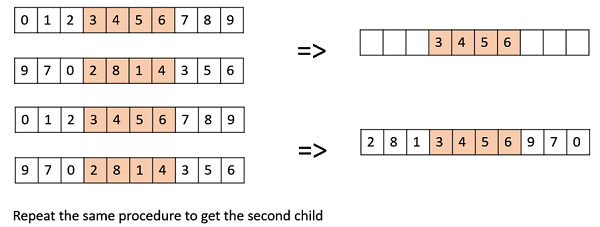
\includegraphics[width=6.25in,height=2.37in]{./media/image16.png}
	\end{Center}
\end{figure}


%%%%%%%%%%%%%%%%%%%% Figure/Image No: 16 Ends here %%%%%%%%%%%%%%%%%%%%

\setlength{\parskip}{8.04pt}
\par


\vspace{\baselineskip}

\vspace{\baselineskip}

\vspace{\baselineskip}
	\item {\fontsize{20pt}{24.0pt}\selectfont Mutation Operators\par}
\end{enumerate}\par

\setlength{\parskip}{7.2pt}
\begin{adjustwidth}{0.03in}{0.03in}
{\fontsize{14pt}{16.8pt}\selectfont \uline{Bit Flip Mutation}\par}\par

\end{adjustwidth}

\begin{adjustwidth}{0.03in}{0.03in}
{\fontsize{11pt}{13.2pt}\selectfont In this bit flip mutation, we select one or more random bits and flip them. This is used for binary encoded GAs.\par}\par

\end{adjustwidth}



%%%%%%%%%%%%%%%%%%%% Figure/Image No: 17 starts here %%%%%%%%%%%%%%%%%%%%

\begin{figure}[H]
	\begin{Center}
		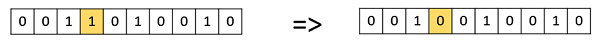
\includegraphics[width=6.25in,height=0.45in]{./media/image17.png}
	\end{Center}
\end{figure}


%%%%%%%%%%%%%%%%%%%% Figure/Image No: 17 Ends here %%%%%%%%%%%%%%%%%%%%

\setlength{\parskip}{8.04pt}
\par


\vspace{\baselineskip}
\setlength{\parskip}{7.2pt}
\begin{adjustwidth}{0.03in}{0.03in}
{\fontsize{14pt}{16.8pt}\selectfont \uline{Random Resetting}\par}\par

\end{adjustwidth}

\begin{adjustwidth}{0.03in}{0.03in}
{\fontsize{11pt}{13.2pt}\selectfont Random Resetting is an extension of the bit flip for the integer representation. In this, a random value from the set of permissible values is assigned to a randomly chosen gene.\par}\par

\end{adjustwidth}


\vspace{\baselineskip}
\begin{adjustwidth}{0.03in}{0.03in}
{\fontsize{14pt}{16.8pt}\selectfont \uline{Swap Mutation}\par}\par

\end{adjustwidth}

\begin{adjustwidth}{0.03in}{0.03in}
{\fontsize{11pt}{13.2pt}\selectfont In swap mutation, we select two positions on the chromosome at random, and interchange the values. This is common in permutation-based encodings.\par}\par

\end{adjustwidth}



%%%%%%%%%%%%%%%%%%%% Figure/Image No: 18 starts here %%%%%%%%%%%%%%%%%%%%

\begin{figure}[H]
	\begin{Center}
		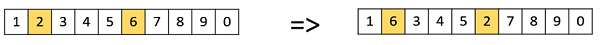
\includegraphics[width=6.25in,height=0.47in]{./media/image18.png}
	\end{Center}
\end{figure}


%%%%%%%%%%%%%%%%%%%% Figure/Image No: 18 Ends here %%%%%%%%%%%%%%%%%%%%

\setlength{\parskip}{8.04pt}
\par


\vspace{\baselineskip}
\setlength{\parskip}{7.2pt}
\begin{adjustwidth}{0.03in}{0.03in}
{\fontsize{14pt}{16.8pt}\selectfont \uline{Scramble Mutation}\par}\par

\end{adjustwidth}

\begin{adjustwidth}{0.03in}{0.03in}
{\fontsize{11pt}{13.2pt}\selectfont Scramble mutation is also popular with permutation representations. In this, from the entire chromosome, a subset of genes is chosen and their values are scrambled or shuffled randomly.\par}\par

\end{adjustwidth}



%%%%%%%%%%%%%%%%%%%% Figure/Image No: 19 starts here %%%%%%%%%%%%%%%%%%%%

\begin{figure}[H]
	\begin{Center}
		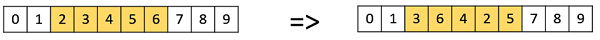
\includegraphics[width=6.25in,height=0.42in]{./media/image19.png}
	\end{Center}
\end{figure}


%%%%%%%%%%%%%%%%%%%% Figure/Image No: 19 Ends here %%%%%%%%%%%%%%%%%%%%

\setlength{\parskip}{8.04pt}
\par


\vspace{\baselineskip}
\setlength{\parskip}{7.2pt}
\begin{adjustwidth}{0.03in}{0.03in}
{\fontsize{14pt}{16.8pt}\selectfont \uline{Inversion Mutation}\par}\par

\end{adjustwidth}

\begin{adjustwidth}{0.03in}{0.03in}
{\fontsize{11pt}{13.2pt}\selectfont In inversion mutation, we select a subset of genes like in scramble mutation, but instead of shuffling the subset, we merely invert the entire string in the subset.\par}\par

\end{adjustwidth}



%%%%%%%%%%%%%%%%%%%% Figure/Image No: 20 starts here %%%%%%%%%%%%%%%%%%%%

\begin{figure}[H]
	\begin{Center}
		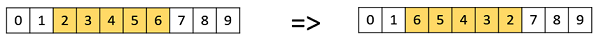
\includegraphics[width=6.25in,height=0.4in]{./media/image20.png}
	\end{Center}
\end{figure}


%%%%%%%%%%%%%%%%%%%% Figure/Image No: 20 Ends here %%%%%%%%%%%%%%%%%%%%

\setlength{\parskip}{8.04pt}
\par


\vspace{\baselineskip}

\vspace{\baselineskip}
\begin{Center}
{\fontsize{28pt}{33.6pt}\selectfont Q4\par}
\end{Center}\par

{\fontsize{14pt}{16.8pt}\selectfont Apply GA based approach to solve an instance of Travelling Salesman problem.\par}\par


\vspace{\baselineskip}
{\fontsize{14pt}{16.8pt}\selectfont \uline{Problem:}\par}\par

Given a set of cities and distance between every pair of cities, the problem is to find the shortest possible route that visits every city exactly once and returns to the starting point.\par


\vspace{\baselineskip}
{\fontsize{14pt}{16.8pt}\selectfont \uline{Pseudo Code:}\par}\par

\begin{enumerate}
	\item Initialize the population randomly.\par

	\item Determine the fitness of the chromosome.\par

	\item Until done repeat: \par

\begin{enumerate}
	\item Select parents.\par

	\item Perform crossover and mutation.\par

	\item Calculate the fitness of the new population.\par

	\item Append it to the gene pool.
\end{enumerate}
\end{enumerate}\par

{\fontsize{14pt}{16.8pt}\selectfont \uline{Trace:}\par}\par

Input Dataset, \par



%%%%%%%%%%%%%%%%%%%% Table No: 2 starts here %%%%%%%%%%%%%%%%%%%%


\begin{table}[H]
 			\centering
\begin{tabular}{p{0.88in}p{0.88in}p{0.88in}p{0.88in}p{0.88in}p{0.88in}}
\hline
%row no:1
\multicolumn{1}{p{0.88in}}{} & 
\multicolumn{1}{p{0.88in}}{0} & 
\multicolumn{1}{p{0.88in}}{1} & 
\multicolumn{1}{p{0.88in}}{2} & 
\multicolumn{1}{p{0.88in}}{3} & 
\multicolumn{1}{p{0.88in}}{4} \\
\hhline{------}
%row no:2
\multicolumn{1}{p{0.88in}}{0} & 
\multicolumn{1}{|p{0.88in}}{0} & 
\multicolumn{1}{|p{0.88in}}{2} & 
\multicolumn{1}{|p{0.88in}}{inf} & 
\multicolumn{1}{|p{0.88in}}{12} & 
\multicolumn{1}{|p{0.88in}|}{5} \\
\hhline{~-----}
%row no:3
\multicolumn{1}{p{0.88in}}{1} & 
\multicolumn{1}{|p{0.88in}}{2} & 
\multicolumn{1}{|p{0.88in}}{0} & 
\multicolumn{1}{|p{0.88in}}{4} & 
\multicolumn{1}{|p{0.88in}}{8} & 
\multicolumn{1}{|p{0.88in}|}{Inf} \\
\hhline{~-----}
%row no:4
\multicolumn{1}{p{0.88in}}{2} & 
\multicolumn{1}{|p{0.88in}}{inf} & 
\multicolumn{1}{|p{0.88in}}{4} & 
\multicolumn{1}{|p{0.88in}}{0} & 
\multicolumn{1}{|p{0.88in}}{3} & 
\multicolumn{1}{|p{0.88in}|}{3} \\
\hhline{~-----}
%row no:5
\multicolumn{1}{p{0.88in}}{3} & 
\multicolumn{1}{|p{0.88in}}{12} & 
\multicolumn{1}{|p{0.88in}}{8} & 
\multicolumn{1}{|p{0.88in}}{3} & 
\multicolumn{1}{|p{0.88in}}{0} & 
\multicolumn{1}{|p{0.88in}|}{10} \\
\hhline{~-----}
%row no:6
\multicolumn{1}{p{0.88in}}{4} & 
\multicolumn{1}{|p{0.88in}}{5} & 
\multicolumn{1}{|p{0.88in}}{inf} & 
\multicolumn{1}{|p{0.88in}}{3} & 
\multicolumn{1}{|p{0.88in}}{10} & 
\multicolumn{1}{|p{0.88in}|}{0} \\
\hhline{~-----}

\end{tabular}
 \end{table}


%%%%%%%%%%%%%%%%%%%% Table No: 2 ends here %%%%%%%%%%%%%%%%%%%%


\vspace{\baselineskip}
Let encoding be in such a way that 012340 means he is travel travelled from 0 to 1 to 2 to 3 to 4 to 0. \par

And the cost of this path will be fitness. Let the Population size be 10. Initial Temperature be 10000. And before mutating each generation, lets sort based on fitness in ascending order. We are going to run this algo for 5 generations.\par

New temperature = 0.9 $\ast$  (Old temperature)\par

Initial Generation, \par

\par

For our mutation, let’s take a 2 random position of a gene in the current population and swap them. \par

This new gene will only get accepted if its fitness is less than its parents, or if its Boltzmann probability is greater than 0.5. \par

So, our current gnome is 043210 with fitness score of 24. The first mutated gene is 043120 with fitness score of infinity. \par

Clearly, the fitness of the child is greater than the parent, therefore we need to calculate the probability. By formula, we get prob = 0. \par

Therefore, we reject this child and calculate another, the next mutated child gnome is 013240 with fitness score of 21. As the child is fitter than the parent, we send them to the next gen. \par

Similarly do for the rest, to show the use of probability, So, our current gnome is 012340 with fitness score of 24. The first mutated gene is 012430 with fitness score of 31. \par

Clearly, the fitness of the child is greater than the parent, therefore we need to calculate the probability. By formula, we get prob = 0.999305. \par

Therefore, we accept this child into the next generation. This way, we get, \par

Gen 1, \par

\par

T\textsubscript{new} = 9000\  -\  Gen 2, \tab \tab \tab \ \ \  T\textsubscript{new}\ =\ 8100  -  Gen 3, \par

\tab \tab \tab \par


\vspace{\baselineskip}
T\textsubscript{new} = 7290\  -\  Gen 4, \tab \tab \tab T\textsubscript{new}\ =\ 6561  -  Gen 5, \par

\tab \tab \tab \par


\vspace{\baselineskip}
It’s clear from the 5th generation that the minimum distance is 21 and 034210 can be one of the possible solutions.\par


\vspace{\baselineskip}

\vspace{\baselineskip}

\vspace{\baselineskip}

\vspace{\baselineskip}

\vspace{\baselineskip}

\vspace{\baselineskip}

\vspace{\baselineskip}
\begin{Center}
{\fontsize{28pt}{33.6pt}\selectfont Q5\par}
\end{Center}\par

{\fontsize{14pt}{16.8pt}\selectfont Understand the working of SLIQ and ARBC classifiers. Give a pseudocode and illustrate the same over a sample dataset of your choice.\par}\par

\begin{enumerate}
	\item {\fontsize{20pt}{24.0pt}\selectfont SLIQ Classifier\par}\par

{\fontsize{14pt}{16.8pt}\selectfont \uline{Introduction:}\par}\par

Supervised Learning in Quest is a decision tree classifier that can handle both numeric and categorical attributes. SLIQ uses a pre-sorting technique in the tree-growth phase to reduce the cost of evaluating numeric attributes. This sorting procedure is integrated with a breadth-first tree growing strategy to enable SLIQ to classify disk-resident datasets. In addition, SLIQ uses a fast sub setting algorithm for determining splits for categorical attributes. SLIQ also uses a new tree-pruning algorithm based on the Minimum Description Length principle. This algorithm is inexpensive, and results in compact and accurate trees. The combination of these techniques enables SLIQ to scale for large data sets and classify data sets with a large number of classes, attributes, and examples.\par

{\fontsize{14pt}{16.8pt}\selectfont \uline{Pseudo Code:}\par}\par

Key Features,\par

\begin{enumerate}
	\item Tree Classifier, handling numeric and categoric attributes\par

	\item Presorting numeric attributes before tree has been built\par

	\item Breadth first growing strategy\par

	\item Goodness test – Gini Index\par

	\item Inexpensive tree pruning algorithm based on Minimum Description Length (MDL)
\end{enumerate}\par

In Presorting, \par

\begin{enumerate}
	\item Eliminate need for sorting data at each node\par

	\item Create sorted list for each numeric attribute\par

	\item Create class list
\end{enumerate}\par

Split Evaluation, \par

EvaluateSplits()\par

For each attribute A do\par

\tab Traverse attribute list of A\par

\tab For each value v in attribute list do\par

\begin{adjustwidth}{1.0in}{0.0in}
Find the corresponding entry in the class list, and hence the corresponding class and the leaf node l\par

\end{adjustwidth}

\begin{adjustwidth}{1.0in}{0.0in}
Update the class histogram in leaf l\par

\end{adjustwidth}

\begin{adjustwidth}{1.0in}{0.0in}
If A is a numeric attribute then\par

\end{adjustwidth}

\begin{adjustwidth}{1.0in}{0.0in}
\tab Compute splitting index for test (A <= v) for l\par

\end{adjustwidth}

\tab If A is a categorical attribute then\par

\tab \tab For each leaf of the tree do\par

\tab \tab \tab Find subset of A with best split\par

Update Class List, \par

UpdateLabels()\par

For each attribute A used in a split do\par

\tab Traverse attribute list of A\par

\tab For each value v in attribute list do\par

\tab \tab Find the corresponding entry in the class list e\par

\tab \tab Find the new class c to which v belongs by applying the splitting test at node referenced\par

\begin{adjustwidth}{0.5in}{0.0in}
from e\par

\end{adjustwidth}

\begin{adjustwidth}{0.5in}{0.0in}
Update the class label for e to c\par

\end{adjustwidth}

\begin{adjustwidth}{0.5in}{0.0in}
Update node referenced in e to the child corresponding to the class c\par

\end{adjustwidth}

{\fontsize{14pt}{16.8pt}\selectfont \uline{Trace:}\par}\par

Training Dataset, \par

\par


\vspace{\baselineskip}
Pre-Sorting and Breadth-First Growth, \par

For numeric attributes, sorting time is the dominant factor when finding the best split at a decision tree node. Therefore, the first technique used in SLIQ is to implement a scheme that eliminates the need to sort the data at each node of the decision tree. Instead, the training data are sorted just once for each numeric attribute at the beginning of the tree growth phase. To achieve this pre-sorting, we use the following data structures. We create a separate list for each attribute of the training data. Additionally, a separate list, called class list, is created for the class labels attached to the examples. An entry in an attribute list has two fields: one contains an attribute value, the other an index into the class list. An entry of the class list also has two fields: one contains a class label, the other a reference to a leaf node of the decision tree. The i\textsuperscript{th} entry of the class list corresponds to the i\textsuperscript{th} example in the training data. Each leaf node of the decision tree represents a partition of the training data, the partition being defined by the conjunction of the predicates on the path from the node to the root. Thus, the class list can at any time identify the partition to which an example belongs. We assume that there is enough memory to keep the class list memory-resident. Attribute lists are written to disk if necessary. Initially, the leaf reference fields of all the entries of the class list are set to point to the root of the decision tree. Then a pass is made over the training data, distributing values of the attributes for each example across all the lists. Each attribute value is also tagged with the corresponding class list index. The attribute lists for the numeric features are then sorted independently.\par

After Presorting, \par

\par

Processing Node Splits, \par

Rather than using a depth-first strategy used in the earlier decision-tree classifiers, we grow trees breadth-first. Consequently, splits for all the leaves of the current tree are simultaneously evaluated in one pass over the data. Figure 4 gives a schematic of the evaluation process. To compute the gini splitting-index for an attribute at a node, we need the frequency distribution of class values in the data partition corresponding to the node. The distribution is accumulated in a class histogram attached with each leaf node. For a numeric attribute, the histogram is a list of pairs of the form ¡class, frequency¿. For a categorical attribute, this histogram is a list of triples of the form ¡attribute value, class, frequency¿. Attribute lists are processed one at a time (recall that the attribute lists can be on disk). For each value IJ in the attribute list for the current attribute A, we find the the corresponding entry in the class list, which yields the corresponding class and the leaf node. We now update the histogram attached with this leaf node. If A is a numeric attribute, we compute at the same time the splitting index for the test A 2 v for this leaf. If A is a categorical attribute, we wait till the attribute list has been completely scanned and then find the subset of A with the best split. Thus, in one traversal of an attribute list, the best split using this attribute is known for all the leaf nodes. Similarly, with one traversal of all of the attribute lists, the best overall split for all of the leaf nodes is known. The best split test is saved with each of the leaf nodes. For our example\par

\par

This figure illustrates the evaluation of splits on the salary attribute for the second level of the decision tree. The example assumes that the data has been initially split on the age attribute using the split age 2 35. The class histograms reflect the distribution of the points at each leaf node as a result of the split. The L values represent the distributions for examples that satisfy the test and R values represent examples that do not satisfy the test. We show how the class histograms are updated as each split is evaluated. The first value in the salary list belongs to node N2. So the first split evaluated is (salary $ \leq $  15) for N2. After this split, the corresponding example (salary 15, class index 2) which satisfies the predicate belongs to the left branch and the rest belong to the right branch. The class histogram of node N2 is updated to reflect this fact. Next, the split (salary 5 40) is evaluated for node N3. After the split, the corresponding example (salary 40, class index 4) belongs to the left branch and the class histogram of node N3 is updated to reflect this fact.\par

Updating the class list, \par

The next step is to create child nodes for each of the leaf nodes and update the class list.\par

Class list updating, \par

\par

As an illustration, above figure shows the class list being updated after the nodes N2 and N3 have been split on the salary attribute. The salary attribute list is being traversed and the class list entry (entry 4) corresponding to the salary value of 40 is being updated. First, the leaf reference in the entry 4 of class list is used to find the node to which the example used to belong (N3 in this case). Then, the split selected at N3 is applied to find the new child to which the example belongs (N6 in this case). The leaf reference field of entry 4 in the class list is updated to reflect the new value. This is how we create the decision tree.\par


\vspace{\baselineskip}

\vspace{\baselineskip}
	\item {\fontsize{20pt}{24.0pt}\selectfont ARBC Classifier\par}
\end{enumerate}\par

{\fontsize{14pt}{16.8pt}\selectfont \uline{Introduction:}\par}\par

Association rule mining was introduced as a way to find associative patterns from market basket data. The market basket data consist of transactions where a transaction is a set of items purchased by a customer. The motivation for applying this data mining approach on market basket data was to learn about buying patterns and use that information in catalog design, and store layout design. Since then, association rule mining has been studied and applied in many other domains (e.g. credit card fraud, network intrusion detection, genetic data analysis). In every domain, there is a need to analyze data to identify patterns associating different attributes. Association rule mining addresses this need. Many association rule mining algorithms have been proposed in the data mining literature. Apriori and FP-growth are two of them.\par


\vspace{\baselineskip}

\vspace{\baselineskip}
{\fontsize{14pt}{16.8pt}\selectfont \uline{Pseudo Code:}\par}\par

Begin\par

minConfidence\par

rules = []\par

freqItemsets = []\par

support = UpperBoundSupport\par

while (support LowerBoundSupport AND rules.size < minNumberOfRules) do\par

\begin{adjustwidth}{0.5in}{0.0in}
L1 = $ \{ $ 1 – item itemsets$ \} $ \par

\end{adjustwidth}

\begin{adjustwidth}{0.5in}{0.0in}
For (k=2; Lk1 6= ) do\par

\end{adjustwidth}

\begin{adjustwidth}{0.5in}{0.0in}
Ck = generateCandidates (L k 1)\par

\end{adjustwidth}

\begin{adjustwidth}{0.5in}{0.0in}
\tab Lk = evaluateCandidates (Ck)\par

\end{adjustwidth}

\begin{adjustwidth}{0.5in}{0.0in}
freqItemsets\  L(k)\par

\end{adjustwidth}

\begin{adjustwidth}{0.5in}{0.0in}
end for\par

\end{adjustwidth}

\begin{adjustwidth}{0.5in}{0.0in}
maxFreqItemsets = genMaxFreqItemset (freqItemsets)\par

\end{adjustwidth}

\begin{adjustwidth}{0.5in}{0.0in}
rules = GenerateAllRules(maxFreqItemsets, minCondfidence)\par

\end{adjustwidth}

\begin{adjustwidth}{0.5in}{0.0in}
support = support – delta\par

\end{adjustwidth}

\begin{adjustwidth}{0.5in}{0.0in}
freqItemsets = []\par

\end{adjustwidth}

end while\par


\vspace{\baselineskip}
R = rules\par

R = sort(R)\par

For each rule r $ \in $  R in sequence do\par

\tab Temp = $ \varnothing $ \par

\tab For each instance d $ \in $  D do\par

\tab If d satisfies the conditions of r then\par

\tab \tab Store d.id in temp and mark r if it correctly classifies d\par

\tab End if\par

End for\par

Find the first rule p in C such that C\textsubscript{p}, the rules in C up to p, has lowest number of errors and drop all the rules\par

Add the default class associated with p to the end of C, and return C\par

End\par


\vspace{\baselineskip}
{\fontsize{14pt}{16.8pt}\selectfont \uline{Trace:}\par}\par

Training Dataset\par



%%%%%%%%%%%%%%%%%%%% Figure/Image No: 21 starts here %%%%%%%%%%%%%%%%%%%%

\begin{figure}[H]
	\begin{Center}
		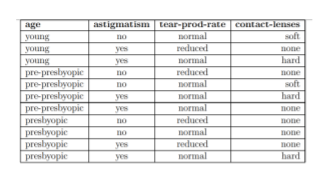
\includegraphics[width=5.97in,height=3.16in]{./media/image31.png}
	\end{Center}
\end{figure}


%%%%%%%%%%%%%%%%%%%% Figure/Image No: 21 Ends here %%%%%%%%%%%%%%%%%%%%

\par

First, Create Associate Rules,\par

For this, we can use any associate rule mining algorithm to mine the classification rule. In associative classification, the focus is to produce association rules that have only a particular attribute in the consequent. These association rules produced are called class association rules (CARs). Associative classification differs from general association rule mining by introducing a constraint as to the attribute that must appear on the consequent of the rule. The CBA-RG algorithm is an extension of the Apriori algorithm. The goal of this algorithm is to find all rule items of the form < condset, y > where condset is a set of items, and y $ \in $  Y, where Y is the set of class labels. The support count of the rule item is the number of instances in the data set D that contain the condset and are labeled with y. Each rule item corresponds to a rule of the form: condset $ \rightarrow $  y.\par

Applying Apriori with support 3, \par


\vspace{\baselineskip}


%%%%%%%%%%%%%%%%%%%% Figure/Image No: 22 starts here %%%%%%%%%%%%%%%%%%%%

\begin{figure}[H]
	\begin{Center}
		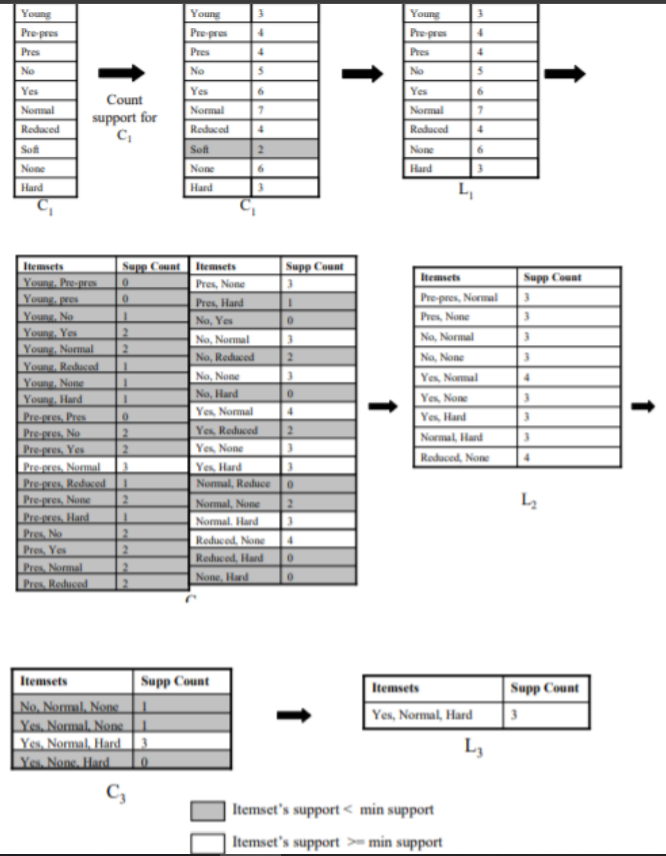
\includegraphics[width=6.62in,height=7.08in]{./media/image32.png}
	\end{Center}
\end{figure}


%%%%%%%%%%%%%%%%%%%% Figure/Image No: 22 Ends here %%%%%%%%%%%%%%%%%%%%

\par

Classifying based on rules,\par

 Rule items that have support greater than or equal to minsup are called frequent rule items, while the others are called infrequent rule items. For all rule items that have the same condset, the one with the highest confidence is selected as the representative of those rule items. The confidence of rule items is calculated to determine if the rule item meets minconf. The set of rules that is selected after checking for support and confidence is called the classification association rules (CARs). Given a model and a new instance whose class is unknown, the problem of predicting the instance’s class using the model is an interesting problem. There is more than one way to use the model to predict the instance’s class. In association rule-based classification models, rules in the model are ordered as follows:\par

\begin{itemize}
	\item if rule ri has greater confidence than rj, then ri precedes rj, or\par

	\item if ri has the same confidence as rj, then the rule with greater support precede the other, or\par

	\item if ri has the same support and the same confidence as rj, then the rule with then smaller number of items in the antecedent will precede, or\par

	\item if ri has the same support, confidence and antecedent size as rj, then the order between the two rules is random.
\end{itemize}\par

\begin{adjustwidth}{0.03in}{0.0in}
Rules of high confidence are thought to be good for classification. Confidence alone may not make a rule very good. For instance, a rule from an instance that appears only once (high confidence but low support) may not be a good rule for classification. Rules with very high confidence and low support are useful in identifying rare events. After Applying apriori, the rules we get are,\par

\end{adjustwidth}

\begin{adjustwidth}{0.03in}{0.0in}
Apriori rules with confidence 0.5, \par

\end{adjustwidth}



%%%%%%%%%%%%%%%%%%%% Figure/Image No: 23 starts here %%%%%%%%%%%%%%%%%%%%

\begin{figure}[H]
	\begin{Center}
		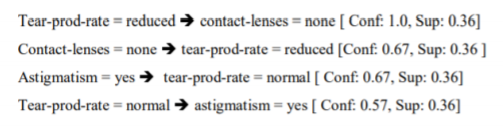
\includegraphics[width=5.24in,height=1.34in]{./media/image33.png}
	\end{Center}
\end{figure}


%%%%%%%%%%%%%%%%%%%% Figure/Image No: 23 Ends here %%%%%%%%%%%%%%%%%%%%

\par


\vspace{\baselineskip}

\vspace{\baselineskip}

\vspace{\baselineskip}

\vspace{\baselineskip}

\vspace{\baselineskip}

\vspace{\baselineskip}

\vspace{\baselineskip}

\vspace{\baselineskip}

\vspace{\baselineskip}

\vspace{\baselineskip}

\vspace{\baselineskip}

\vspace{\baselineskip}

\vspace{\baselineskip}
\begin{Center}
{\fontsize{28pt}{33.6pt}\selectfont Q6\par}
\end{Center}\par

{\fontsize{14pt}{16.8pt}\selectfont Define sequence pattern mining and understand the working of \par}\par

{\fontsize{14pt}{16.8pt}\selectfont i) GSP\par}\par

{\fontsize{14pt}{16.8pt}\selectfont ii) Prefix-Span algorithms.\par}\par

{\fontsize{14pt}{16.8pt}\selectfont Give a pseudocode and illustrate the same over a sample dataset of your choice.\par}\par


\vspace{\baselineskip}
{\fontsize{14pt}{16.8pt}\selectfont \uline{Sequence Pattern Mining}\par}\par

{\fontsize{14pt}{16.8pt}\selectfont \uline{Introduction:}\par}\par

Sequential Pattern Mining is the mining of frequently occurring ordered events or subsequences as pattern in sequence database.\par

A Sequence Database stores a number of records, where all records are sequences of ordered events, with or without concrete notions of time\par

Sequential Patterns are used for targeted marketing and customer retention\par


\vspace{\baselineskip}
\begin{enumerate}
	\item {\fontsize{20pt}{24.0pt}\selectfont GSP\par}\par

{\fontsize{14pt}{16.8pt}\selectfont \uline{Introduction:}\par}\par

The Generalized Sequence Pattern algorithm was created from a simpler algorithm for mining sequences, but it has some extra bells and whistles added so it can be more flexible for different situations.\par

{\fontsize{14pt}{16.8pt}\selectfont \uline{Pseudo Code:}\par}\par

F\textsubscript{1} = the set of frequent 1-sequence\par

\ \  k=2,\par

\ \  do while Fk-1 != Null;\par

\ \ \ \ \ \  Generate candidate sets C\textsubscript{k} (set of candidate k-sequences);\par

\ \ \ \ \ \  For all input sequences s in the database D\par

\ \ \ \ \ \  do\par

\ \ \ \ \ \ \ \ \ \  Increment count of all a in C\textsubscript{k} if s supports a\par

\ \ \ \ \ \  End do\par

\ \ \ \ \ \  F\textsubscript{k} = $ \{ $ a $ \in $  C\textsubscript{k} such that its frequency exceeds the threshold$ \} $ \par

\ \ \ \ \ \  k = k+1;\par

\ \  End do\par

\ \  Result = Set of all frequent sequences is the union of all F\textsubscript{k}'s\par


\vspace{\baselineskip}
{\fontsize{14pt}{16.8pt}\selectfont \uline{Trace:}\par}\par

Input Data\par



%%%%%%%%%%%%%%%%%%%% Table No: 3 starts here %%%%%%%%%%%%%%%%%%%%


\begin{table}[H]
 			\centering
\begin{tabular}{p{1.96in}p{1.96in}p{1.96in}}
\hline
%row no:1
\multicolumn{1}{|p{1.96in}}{Transaction ID} & 
\multicolumn{1}{|p{1.96in}}{Customer ID} & 
\multicolumn{1}{|p{1.96in}|}{Items} \\
\hhline{---}
%row no:2
\multicolumn{1}{|p{1.96in}}{1} & 
\multicolumn{1}{|p{1.96in}}{1} & 
\multicolumn{1}{|p{1.96in}|}{A} \\
\hhline{---}
%row no:3
\multicolumn{1}{|p{1.96in}}{2} & 
\multicolumn{1}{|p{1.96in}}{1} & 
\multicolumn{1}{|p{1.96in}|}{B} \\
\hhline{---}
%row no:4
\multicolumn{1}{|p{1.96in}}{3} & 
\multicolumn{1}{|p{1.96in}}{1} & 
\multicolumn{1}{|p{1.96in}|}{A} \\
\hhline{---}
%row no:5
\multicolumn{1}{|p{1.96in}}{4} & 
\multicolumn{1}{|p{1.96in}}{2} & 
\multicolumn{1}{|p{1.96in}|}{B} \\
\hhline{---}
%row no:6
\multicolumn{1}{|p{1.96in}}{5} & 
\multicolumn{1}{|p{1.96in}}{2} & 
\multicolumn{1}{|p{1.96in}|}{A} \\
\hhline{---}
%row no:7
\multicolumn{1}{|p{1.96in}}{6} & 
\multicolumn{1}{|p{1.96in}}{2} & 
\multicolumn{1}{|p{1.96in}|}{B} \\
\hhline{---}

\end{tabular}
 \end{table}


%%%%%%%%%%%%%%%%%%%% Table No: 3 ends here %%%%%%%%%%%%%%%%%%%%


\vspace{\baselineskip}
First we prune Items with less support than threshold\par

Let threshold = 1\par

A – 3 > 1\par

B – 3 > 1\par

Now, get the sequences for each customer\par



%%%%%%%%%%%%%%%%%%%% Table No: 4 starts here %%%%%%%%%%%%%%%%%%%%


\begin{table}[H]
 			\centering
\begin{tabular}{p{3.05in}p{3.05in}}
\hline
%row no:1
\multicolumn{1}{|p{3.05in}}{Customer ID} & 
\multicolumn{1}{|p{3.05in}|}{Sequence} \\
\hhline{--}
%row no:2
\multicolumn{1}{|p{3.05in}}{1} & 
\multicolumn{1}{|p{3.05in}|}{ABA} \\
\hhline{--}
%row no:3
\multicolumn{1}{|p{3.05in}}{2} & 
\multicolumn{1}{|p{3.05in}|}{BAB} \\
\hhline{--}

\end{tabular}
 \end{table}


%%%%%%%%%%%%%%%%%%%% Table No: 4 ends here %%%%%%%%%%%%%%%%%%%%


\vspace{\baselineskip}
L1 = $ \{ $ A, B$ \} $ \par

We generate C2, \par

C2 = $ \{ $ AA, BB, AB, BA$ \} $ \par

Supports are, \par

AA – 1 – (A)B(A) in CID 1\par

BB – 1 – (B)A(B) in CID 2\par

AB – 2 – (AB)A and B(AB) in CID 1 and 2\par

BA – 2 – A(BA) and (BA)B in CID 1 and 2\par

All > 1 (Threshold)\par

L2 = $ \{ $ AA, AB, BA, BB$ \} $ \par

We generate C3, \par

C3 = $ \{ $ AAA, AAB, ABA, ABB, BAA, BAB, BBA, BBB$ \} $ \par

Supports are, \par

AAA – 0\par

AAB – 0\par

ABA – 1 >= 1\par

ABB – 0\par

BAA – 0\par

BAB – 1 >= 1\par

BBA – 0\par

BBB – 0\par

So, L3 = $ \{ $ ABA, BAB$ \} $ \par

So, frequent sequences are $ \{ $ A, B, AA, AB, BA, BB, ABA, BAB$ \} $ \par


\vspace{\baselineskip}
	\item {\fontsize{20pt}{24.0pt}\selectfont Prefix Span Algorithm\par}
\end{enumerate}\par

{\fontsize{14pt}{16.8pt}\selectfont \uline{Introduction:}\par}\par

\setlength{\parskip}{0.0pt}
A pattern-growth method based on projection is used in Prefix Span algorithm for mining sequential patterns. The basic idea behind this method is, rather than projecting sequence databases by evaluating the frequent occurrences of sub-sequences, the projection is made on frequent prefix. This helps to reduce the processing time which ultimately increases the algorithm efficiency.\par


\vspace{\baselineskip}
\setlength{\parskip}{8.04pt}
{\fontsize{14pt}{16.8pt}\selectfont \uline{Pseudo Code:}\par}\par

\textbf{Input:} A sequence database S, and the minimum support threshold min\_sup \par

\textbf{Output:} The complete set of sequential patterns \par

\textbf{Parameters: }\par

\begin{enumerate}
	\item $ \alpha $ : sequential pattern, \par

	\item l: the length of $ \alpha $ ; \par

	\item S$ \vert $ $ \alpha $ : the $ \alpha $ -projected database, if $ \alpha $  $ \neq $ <>; otherwise; the sequence database S
\end{enumerate}\par

Algorithm\par

PrefixSpan($ \alpha $ , l, S$ \vert $ $ \alpha $ )\par

\begin{enumerate}
	\item Scan S$ \vert $ $ \alpha $  once, find the set of frequent items b such that: \par

\begin{enumerate}
	\item b can be assembled to the last element of $ \alpha $  to form a sequential pattern; or \par

	\item can be appended to $ \alpha $  to form a sequential pattern.\par


\end{enumerate}
	\item For each frequent item b, append it to $ \alpha $  to form a sequential pattern $ \alpha $ ’, and output $ \alpha $ ’;\par

	\item For each $ \alpha $ ’, construct $ \alpha $ ’-projected database S$ \vert $ $ \alpha $ ’, and call PrefixSpan($ \alpha $ ’, l+1, S$ \vert $ $ \alpha $ ’).
\end{enumerate}\par


\vspace{\baselineskip}{\fontsize{14pt}{16.8pt}\selectfont \uline{Trace:}\par}\par

Let minsup be 2, \par

Dataset, \par



%%%%%%%%%%%%%%%%%%%% Figure/Image No: 24 starts here %%%%%%%%%%%%%%%%%%%%

\begin{figure}[H]
	\begin{Center}
		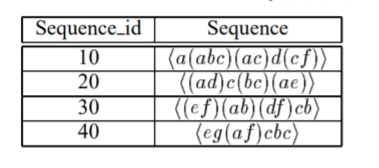
\includegraphics[width=3.95in,height=1.75in]{./media/image34.png}
	\end{Center}
\end{figure}


%%%%%%%%%%%%%%%%%%%% Figure/Image No: 24 Ends here %%%%%%%%%%%%%%%%%%%%

\par

Find length -1 sequential patterns, \par

Scan the database once to find all frequent items in sequences. Each of these frequent items is a length-1 sequential pattern. They are: \par

< a >: 4, < b >: 4, < c >: 4, < d >: 3, < e >: 3, < f >: 3\par

where < prefix >: count.\par

Divide search space\par

The complete set of sequential patterns can be partitioned into the following six subsets according to the six prefixes: (1) the ones having prefix < a > ; ... ; and (6) the ones having prefix < f >.\par

Find subsets of sequential patterns\par

The subsets of sequential patterns can be mined by constructing corresponding projected databases and mine each recursively. The projected databases as well as sequential patterns found in them are listed in Table 2, while the mining process is explained as follows, First, let us find sequential patterns having prefix < a >. Only the sequences containing < a > should be collected.ted. Moreover, in a sequence containing < a >, only the subsequence prefixed with the first occurrence of < a >, should be considered. For example, in sequence < (ef)(ab)(df)cb > only the subsequence < ( b)(df)cb > should be considered for mining sequential patterns having prefix < a >. Notice that (b) means that the last element in the prefix, which is a, together with b, form one element. As another example, only the subsequence < (abc)(ac)d(cf) > of sequence < a(abc)(ac)d(cf) > is considered. For our example,\par

Sequences in S containing < a > are projected wrt < a > to form the < a > - projected database, which consists of four postfix sequences : < (abc)(ac)d(cf) >, < ( d)c(bc)(ae) >, < ( b)(df)cb > and < ( f)cbc >. By scanning < a >-projected database once, all the lenght-2 sequential patterns having prefix < a > can be found.\par

They are: < aa >: 2, < ab >: 4, < (ab) >: 2, < ac >: 4, < ad >: 2, < af >: 2.\par

Recursively, all sequential having patterns prefix < a > can be partitioned into 6 subsets: (1) those having prefix < aa >, (2) those having prefix < ab >, . . ., and finally, (6) those having prefix < af >. These subsets can be mined by constructing respective projected databases and mining each recursively.\par

The\ <\ aa\ >\ -projected\ database\ consists of only one non-empty (postfix) subsequences having prefix       < aa > : < ( bc)(ac)d(cf) >. Since there is no hope to generate any frequent subsequence from a single sequence, the processing of < aa >-projected database terminates.\par

The < ab > -projected database consists of three postfix sequences: < ( c)(ac)d(cf) >, < ( c)a > and < c >.\par

Recursively mining < ab > -projected database returns fours sequential patterns: < ( c) >, < ( c)a >, < a > and < c > (i.e. < a(bc) >, < a(bc)a >, < aba > and < abc >).\par

The < (ab) > projected sequence only consist of two sequence, < ( c)(ac)d(cf) > and < (df)c >, which leads to the finding of the following sequential patterns having prefix < (ab) > : < c >, < d >, < f > and < dc >.\par

The < ac > $-$ , < ad > $-$  and < af > $-$  projected databases can be constructed and recursively mined similarly. The sequential patterns found are shown in figure.\par

Similarly, we can find sequential patterns having prefix < b >, < c >, < d >, < e > and < f > by constructing < b, > $-$ , < c > $-$ , < d > $-$ , < e > $-$  and < f > $-$  projected databases and mining them respectively. The projected databases are shown in figure.\par

Projected Databases and Sequential Patterns, \par



%%%%%%%%%%%%%%%%%%%% Figure/Image No: 25 starts here %%%%%%%%%%%%%%%%%%%%

\begin{figure}[H]
	\begin{Center}
		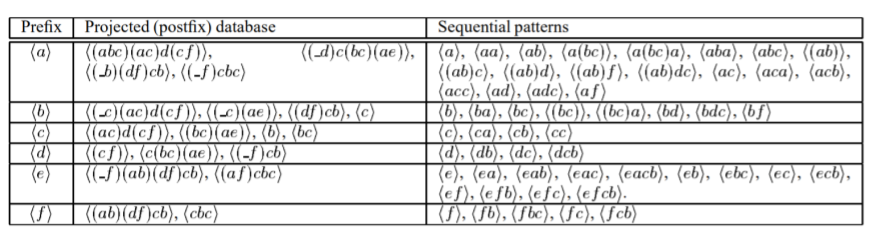
\includegraphics[width=6.5in,height=1.79in]{./media/image35.png}
	\end{Center}
\end{figure}


%%%%%%%%%%%%%%%%%%%% Figure/Image No: 25 Ends here %%%%%%%%%%%%%%%%%%%%

\par


\vspace{\baselineskip}

\vspace{\baselineskip}

\vspace{\baselineskip}
\begin{Center}
{\fontsize{28pt}{33.6pt}\selectfont Q7\par}
\end{Center}\par

{\fontsize{14pt}{16.8pt}\selectfont Understand the schemata theorem of GA (relevance of selection/crossover/mutation with the 3 components of the schema theorem. Apply the theorem to the optimization function f(x)= x3-2x2+x. Check whether the empirical results obtained earlier in assignment-I matches with the theorem.\par}\par

{\fontsize{14pt}{16.8pt}\selectfont \uline{Introduction:}\par}\par

\setlength{\parskip}{6.0pt}
Using the established methods and genetic operators of genetic algorithms, the schema theorem states that short, low-order schemata with above-average fitness increase exponentially in successive generations. Expressed as an equation:\par

 \[ E \left( m \left( H, t+1 \right)  \right)  \geq  \frac{m \left( \text{H, t} \right) f \left( H \right) }{a_{t}} \left[ 1-p \right]  \] \par

Here  \( m \left( \text{H, t} \right) ~ \) $ \{ $ $\textbackslash$ displaystyle m(H,t)$ \} $ is the number of strings belonging to schema $ \{ $ $\textbackslash$ displaystyle H$ \} $ H at generation $ \{ $ $\textbackslash$ displaystyle t$ \} $ t, $ \{ $ $\textbackslash$ displaystyle f(H)$ \} $  \( ~f \left( H \right)  \)  is the \textit{observed} average fitness of schema $ \{ $ $\textbackslash$ displaystyle H$ \} $ H and $ \{ $ $\textbackslash$ displaystyle a\_$ \{ $ t$ \} $ $ \} $  \( a_{t} \)  is the \textit{observed} average fitness at generation $ \{ $ $\textbackslash$ displaystyle t$ \} $ t. The probability of disruption $ \{ $ $\textbackslash$ displaystyle p$ \} $ p is the probability that crossover or mutation will destroy the schema $ \{ $ $\textbackslash$ displaystyle H$ \} $ H. It can be expressed as:\par

 \[ p=\frac{ \delta  \left( H \right) }{l-1}p_{c}+o \left( H \right) p_{m} \] \par

\setlength{\parskip}{1.2pt}
$ \{ $ $\textbackslash$ displaystyle p=$ \{ $ $\textbackslash$ delta (H) $\textbackslash$ over l-1$ \} $ p\_$ \{ $ c$ \} $ +o(H)p\_$ \{ $ m$ \} $ $ \} $ where $ \{ $ $\textbackslash$ displaystyle o(H)$ \} $  \(  o \left( H \right)  \)  is the order of the schema, $ \{ $ $\textbackslash$ displaystyle l$ \} $ l is the length of the code, $ \{ $ $\textbackslash$ displaystyle p\_$ \{ $ m$ \} $ $ \} $  \( ~p_{m} \)  is the probability of mutation and $ \{ $ $\textbackslash$ displaystyle p\_$ \{ $ c$ \} $ $ \} $  \( p_{c} \)  is the probability of crossover. So, a schema with a shorter defining length $ \{ $ $\textbackslash$ displaystyle $\textbackslash$ delta (H)$ \} $  \(   \delta  \left( H \right)  \)  is less likely to be disrupted.\par


\vspace{\baselineskip}
\setlength{\parskip}{8.04pt}
{\fontsize{14pt}{16.8pt}\selectfont \uline{Implications of Schema Theorem:}\par}\par

Schemas, like families, need nourishment and encouragement and careful protective management\par

\begin{enumerate}
	\item The more bits in your building block family the more likely one is to go off the rails (causing great frustration and heartache).\par

	\item Genes living far apart are prone to breaking up.\par

	\item Conducting a constructive relationship at a distance is hard.\par

	\item Best results achieved by the family unit huddled together in consecutive positions.
\end{enumerate}\par

{\fontsize{14pt}{16.8pt}\selectfont \uline{Applications of Schema Theorem:}\par}\par

The schema theorem is more applicable at the early stages of a search rather than at the end. Schema theorem indicates that fitter than average schemas are rewarded. The fitter the schema the more it is rewarded.\par

\begin{enumerate}
	\item Reward is immediate: you see it in the next generation\par

	\item Should alert us to one danger immediately\par

	\item Premature converge of the population
\end{enumerate}\par

{\fontsize{14pt}{16.8pt}\selectfont \uline{Trace:}\par}\par

The optimization function is, \par

 \[ x^{3}-2x^{2}+x \] \par

The constraint on x is \par

 \[ x~ \in   \left[ 0, 31 \right]  \] \par

Choose Encoding, \par

As x max is 31, we use 5-bit binary representation of x\par

Generate Schema, \par

The randomly generated schemas are: \par

[’01$\ast$ 0$\ast$ ’, ’000$\ast$ 0’, ’0$\ast$ 1$\ast$ $\ast$ ’, ’$\ast$ 0$\ast$ 00’, ’10$\ast$ 11’, ’01$\ast$ $\ast$ 1’]\par

Calculate the average fitness of each schema, \par

The average fitness of a schema is the average of all the instances of that schema. In our case, the fitness of each schema is: \par

[1073.0, 2147.0, 1680.25, 6074.5, 20793.0, 12018.5]\par

Select schema for crossover, \par

Schemas are selected in Russian roulette fashion with probabilities of getting selected being defined as:\par

 \[ p \left( x_{i} \right) = \frac{F \left( x_{i} \right) }{ \sum _{j=1}^{N}F \left( x_{i} \right) } \] \par

In our case, the probability of each schema getting selected are:\par

[0.025, 0.049, 0.038, 0.139, 0.475, 0.274] \par

And the schema chosen for crossover are:\par

[’10$\ast$ 11’ ’000$\ast$ 0’ ’10$\ast$ 11’ ’10$\ast$ 11’ ’10$\ast$ 11’ ’10$\ast$ 11’]\par

Crossover, \par

Randomly pair up the schemas selected for crossover: In our case:\par

10$\ast$ 11 and 10$\ast$ 11\par

000$\ast$ 0 and 10$\ast$ 11\par

10$\ast$ 11 and 10$\ast$ 11\par

We are using single point crossover and the offspring generated are:\par

[’01$\ast$ 0$\ast$ ’, ’00$\ast$ 11’, ’10$\ast$ 11’, ’100$\ast$ 0’, ’10$\ast$ 11’, ’01$\ast$ $\ast$ 1’]\par

Mutation, \par

For mutation, we define a probability of mutation, pm and we go through each gene of the chromosome and mutate them.\par

In our case, p\textsubscript{m} = 0.02.\par

For schema bit with ’$\ast$ ’, mutation makes no difference, so we may not see any mutation. \par

After mutation, our schemas are:\par

[’01$\ast$ 0$\ast$ ’, ’00$\ast$ 11’, ’10$\ast$ 11’, ’100$\ast$ 0’, ’10$\ast$ 11’, ’01$\ast$ $\ast$ 1’]\par

Repeat, \par

Repeat Selection, Crossover and Mutation on the schemas until there is no improvement in the average fitness of the generation.\par

In our case, that is:\par

[’11$\ast$ $\ast$ 1’, ’01$\ast$ 11’, ’10$\ast$ $\ast$ 1’, ’10$\ast$ 11’, ’00$\ast$ 11’, ’01$\ast$ $\ast$ 1’]\par

Perform GA on the schema population, \par

Now that we have the best schemas, create a population with all the instances of all the schemas in the final generation and apply normal ga to this population.\par

In our case, after applying ga to the best schema instance population the optimal solution is: ’11111’\par


\vspace{\baselineskip}

\vspace{\baselineskip}

\vspace{\baselineskip}

\vspace{\baselineskip}

\vspace{\baselineskip}

\vspace{\baselineskip}

\vspace{\baselineskip}

\vspace{\baselineskip}

\vspace{\baselineskip}

\vspace{\baselineskip}

\vspace{\baselineskip}

\vspace{\baselineskip}
\begin{Center}
{\fontsize{28pt}{33.6pt}\selectfont Q8\par}
\end{Center}\par

{\fontsize{14pt}{16.8pt}\selectfont Understand the working of linear and non-linear regression models. Give a pseudocode and illustrate the same over a sample dataset of your choice.\par}\par


\vspace{\baselineskip}
\begin{enumerate}
	\item {\fontsize{20pt}{24.0pt}\selectfont Linear Regression\par}\par

{\fontsize{14pt}{16.8pt}\selectfont \uline{Introduction:}\par}\par

Linear Regression is a statistical approach to modelling the relationship between an input and output as a linear relationship.\par

Given a data set  \(  \{ y_{i},~x_{i1},~x_{i2},  \ldots , x_{ip} \}  \)  of n statistical units, a linear regression model assumes that the relationship between the dependent variable y and the p-vector of regressors x is linear. This relationship is modelled through a disturbance term or error variable \textit{\textcolor[HTML]{202122}{$ \varepsilon $  -}}\textcolor[HTML]{202122}{ an unobserved random variable that adds ‘noise’ to the linear relationship between the dependent variable and regressors. Thus, the model takes the form, }\par

 \[ y_{i}=  \beta _{0}+  \beta _{1}x_{i1}+ \ldots +  \beta _{p}x_{ip}+  \varepsilon _{i} \] \par

 \[ i=1,  \ldots , n \] \par

Where \textsuperscript{T} denotes the transpose, so that  \( x_{i}^{T} \beta  \) \textbf{\textcolor[HTML]{222222}{ }}\textcolor[HTML]{222222}{is the inner product between vectors  \( x_{i} \) } and  \(  \beta  \) \textcolor[HTML]{222222}{.}\par

{\fontsize{14pt}{16.8pt}\selectfont \textcolor[HTML]{222222}{\uline{Pseudo Code:}}\par}\par

\begin{enumerate}
	\item \textcolor[HTML]{222222}{Read Number of Data (n)}\par

	\item \textcolor[HTML]{222222}{For i=1 to n:}\par

\textcolor[HTML]{222222}{\ \  Read Xi and Yi}\par

\textcolor[HTML]{222222}{\ \  Next i}\par

	\item \textcolor[HTML]{222222}{Initialize:}\par

\textcolor[HTML]{222222}{\ \ \ \  \tab sumX = 0}\par

\textcolor[HTML]{222222}{\ \ \ \  \tab sumX2 = 0}\par

\textcolor[HTML]{222222}{\ \ \ \  \tab sumY = 0}\par

\textcolor[HTML]{222222}{\ \ \ \  \tab sumXY = 0}\par

	\item \textcolor[HTML]{222222}{Calculate Required Sum}\par

\textcolor[HTML]{222222}{\  \tab  For i=1 to n:}\par

\textcolor[HTML]{222222}{\ \ \ \  \tab  \tab sumX = sumX + Xi}\par

\textcolor[HTML]{222222}{\ \ \ \  \tab \tab sumX2 = sumX2 + Xi $\ast$  Xi}\par

\textcolor[HTML]{222222}{\ \ \ \  \tab \tab sumY = sumY + Yi}\par

\textcolor[HTML]{222222}{\ \ \  \tab \tab  sumXY = sumXY + Xi $\ast$  Yi}\par

\textcolor[HTML]{222222}{\ \  \tab \tab Next i}\par

	\item \textcolor[HTML]{222222}{Calculate Required Constant a and b of y = a + bx:}\par

\textcolor[HTML]{222222}{b = (n $\ast$  sumXY - sumX $\ast$  sumY)/(n$\ast$ sumX2 - sumX $\ast$  sumX)}\par

\textcolor[HTML]{222222}{a = (sumY - b$\ast$ sumX)/n}\par


\vspace{\baselineskip}
	\item \textcolor[HTML]{222222}{Display value of a and b}
\end{enumerate}\par


\vspace{\baselineskip}
{\fontsize{14pt}{16.8pt}\selectfont \textcolor[HTML]{222222}{\uline{Trace:}}\par}\par

\textcolor[HTML]{222222}{For sample data, }\par

\textcolor[HTML]{222222}{Suppose actual line parameters are}\par

\textcolor[HTML]{222222}{Y = mX + c}\par

\textcolor[HTML]{222222}{Where m = slope = 5}\par

\textcolor[HTML]{222222}{C = intercept = 10}\par

\textcolor[HTML]{222222}{N = 5}\par



%%%%%%%%%%%%%%%%%%%% Table No: 5 starts here %%%%%%%%%%%%%%%%%%%%


\begin{table}[H]
 			\centering
\begin{tabular}{p{3.05in}p{3.05in}}
\hline
%row no:1
\multicolumn{1}{|p{3.05in}}{\textcolor[HTML]{222222}{X}} & 
\multicolumn{1}{|p{3.05in}|}{\textcolor[HTML]{222222}{Y}} \\
\hhline{--}
%row no:2
\multicolumn{1}{|p{3.05in}}{\textcolor[HTML]{222222}{1}} & 
\multicolumn{1}{|p{3.05in}|}{\textcolor[HTML]{222222}{16}} \\
\hhline{--}
%row no:3
\multicolumn{1}{|p{3.05in}}{\textcolor[HTML]{222222}{2}} & 
\multicolumn{1}{|p{3.05in}|}{\textcolor[HTML]{222222}{19}} \\
\hhline{--}
%row no:4
\multicolumn{1}{|p{3.05in}}{\textcolor[HTML]{222222}{3}} & 
\multicolumn{1}{|p{3.05in}|}{\textcolor[HTML]{222222}{26}} \\
\hhline{--}
%row no:5
\multicolumn{1}{|p{3.05in}}{\textcolor[HTML]{222222}{4}} & 
\multicolumn{1}{|p{3.05in}|}{\textcolor[HTML]{222222}{32}} \\
\hhline{--}
%row no:6
\multicolumn{1}{|p{3.05in}}{\textcolor[HTML]{222222}{5}} & 
\multicolumn{1}{|p{3.05in}|}{\textcolor[HTML]{222222}{36}} \\
\hhline{--}

\end{tabular}
 \end{table}


%%%%%%%%%%%%%%%%%%%% Table No: 5 ends here %%%%%%%%%%%%%%%%%%%%


\vspace{\baselineskip}
\textcolor[HTML]{222222}{Now, we calculate sums, }\par

\textcolor[HTML]{222222}{sumX = 1 + 2 + 3 + 4 + 5 = 15}\par

\textcolor[HTML]{222222}{sumY = 16 + 19 + 26 + 32 + 36 = 129}\par

\textcolor[HTML]{222222}{sumX2 = 1 + 4 + 9 + 16 + 25 = 55}\par

\textcolor[HTML]{222222}{sumXY = 16 + 38 + 78 + 128 + 180 = 440}\par

\textcolor[HTML]{222222}{Now, we find parameters, }\par

\textcolor[HTML]{222222}{m = (N $\ast$  sumXY - sumX $\ast$  sumY)/(N$\ast$ sumX2 - sumX $\ast$  sumX) = (5$\ast$ 440 – 15$\ast$ 129) / (5$\ast$ 55 – 15$\ast$ 15)}\par

\textcolor[HTML]{222222}{= 5.3}\par

\textcolor[HTML]{222222}{c = (sumY - m$\ast$ sumX)/N = (129 – 5.3$\ast$ 15) / 5 = 9.9}\par

\textcolor[HTML]{222222}{So, Evaluation, }\par



%%%%%%%%%%%%%%%%%%%% Table No: 6 starts here %%%%%%%%%%%%%%%%%%%%


\begin{table}[H]
 			\centering
\begin{tabular}{p{1.96in}p{1.96in}p{1.96in}}
\hline
%row no:1
\multicolumn{1}{|p{1.96in}}{} & 
\multicolumn{1}{|p{1.96in}}{\textcolor[HTML]{222222}{Actual}} & 
\multicolumn{1}{|p{1.96in}|}{\textcolor[HTML]{222222}{Model}} \\
\hhline{---}
%row no:2
\multicolumn{1}{|p{1.96in}}{\textcolor[HTML]{222222}{Slope}} & 
\multicolumn{1}{|p{1.96in}}{\textcolor[HTML]{222222}{5}} & 
\multicolumn{1}{|p{1.96in}|}{\textcolor[HTML]{222222}{5.3}} \\
\hhline{---}
%row no:3
\multicolumn{1}{|p{1.96in}}{\textcolor[HTML]{222222}{Intercept}} & 
\multicolumn{1}{|p{1.96in}}{\textcolor[HTML]{222222}{10}} & 
\multicolumn{1}{|p{1.96in}|}{\textcolor[HTML]{222222}{9.9}} \\
\hhline{---}

\end{tabular}
 \end{table}


%%%%%%%%%%%%%%%%%%%% Table No: 6 ends here %%%%%%%%%%%%%%%%%%%%


\vspace{\baselineskip}
\textcolor[HTML]{222222}{Larger Dataset, }\par

\textcolor[HTML]{222222}{Input Data}\par



%%%%%%%%%%%%%%%%%%%% Figure/Image No: 26 starts here %%%%%%%%%%%%%%%%%%%%

\begin{figure}[H]
	\begin{Center}
		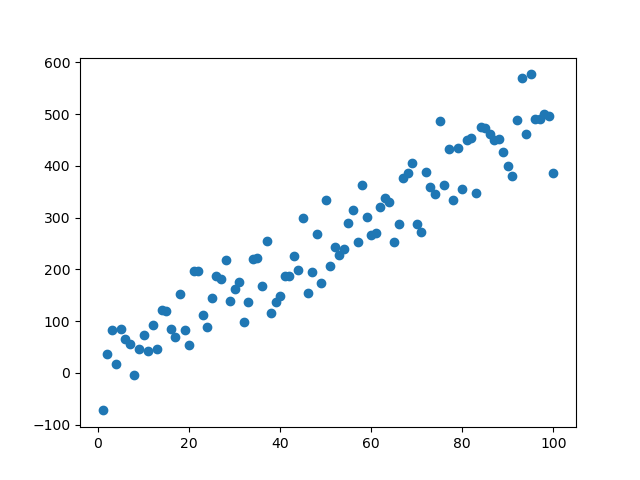
\includegraphics[width=6.4in,height=4.81in]{./media/image36.png}
	\end{Center}
\end{figure}


%%%%%%%%%%%%%%%%%%%% Figure/Image No: 26 Ends here %%%%%%%%%%%%%%%%%%%%

\par


\vspace{\baselineskip}

\vspace{\baselineskip}

\vspace{\baselineskip}

\vspace{\baselineskip}

\vspace{\baselineskip}

\vspace{\baselineskip}

\vspace{\baselineskip}
\textcolor[HTML]{222222}{Output Model}\par



%%%%%%%%%%%%%%%%%%%% Figure/Image No: 27 starts here %%%%%%%%%%%%%%%%%%%%

\begin{figure}[H]
	\begin{Center}
		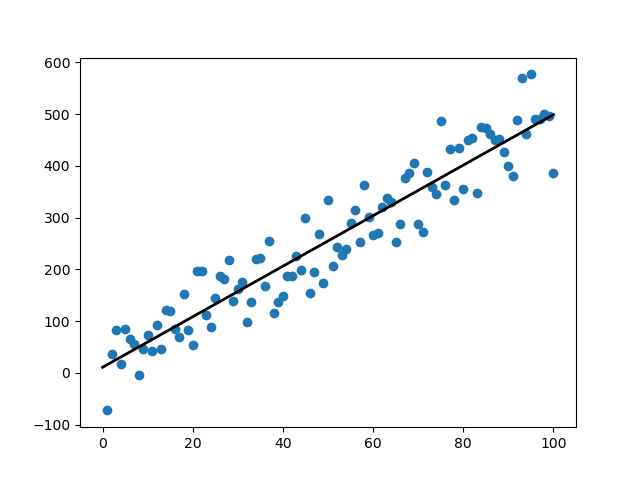
\includegraphics[width=6.4in,height=4.81in]{./media/image37.png}
	\end{Center}
\end{figure}


%%%%%%%%%%%%%%%%%%%% Figure/Image No: 27 Ends here %%%%%%%%%%%%%%%%%%%%

\par

\textcolor[HTML]{222222}{Parameters:}\par

\textcolor[HTML]{222222}{Slope: Actual: 5 - Predicted: 4.880934505955754}\par

\textcolor[HTML]{222222}{Intercept: Actual: 10 - Predicted: 10.804514757031138}\par

\textcolor[HTML]{222222}{Predictions:}\par

\textcolor[HTML]{222222}{X: 12.3 Actual Y: 71.5 - Predicted Y: 70.84000918028691}\par

\textcolor[HTML]{222222}{X: 10.1 Actual Y: 60.5 - Predicted Y: 60.10195326718424}\par

\textcolor[HTML]{222222}{X: 25.2 Actual Y: 136.0 - Predicted Y: 133.80406430711614}\par


\vspace{\baselineskip}

\vspace{\baselineskip}

\vspace{\baselineskip}

\vspace{\baselineskip}

\vspace{\baselineskip}
	\item {\fontsize{20pt}{24.0pt}\selectfont \textcolor[HTML]{222222}{Logistic Regression}\par}
\end{enumerate}\par

{\fontsize{14pt}{16.8pt}\selectfont \textcolor[HTML]{222222}{\uline{Introduction:}}\par}\par

\textcolor[HTML]{202122}{Logistic regression is a }statistical model\textcolor[HTML]{202122}{ that in its basic form uses a }logistic function\textcolor[HTML]{202122}{ to model a }binary\textcolor[HTML]{202122}{ }dependent variable\textcolor[HTML]{202122}{, although many more complex }extensions\textcolor[HTML]{202122}{ exist. In }regression analysis\textcolor[HTML]{202122}{, \textbf{logistic regression} (or \textbf{logit regression}) is }estimating\textcolor[HTML]{202122}{ the parameters of a logistic model (a form of }binary regression\textcolor[HTML]{202122}{).}\par

{\fontsize{14pt}{16.8pt}\selectfont \textcolor[HTML]{202122}{\uline{Pseudo Code:}}\par}\par

\textcolor[HTML]{202122}{Given Dataset, first we fit the logistic regression model to the train data.}\par

\begin{enumerate}
	\item Initialize the parameters\par

	\item Repeat $ \{ $ \\
 \tab Make a prediction on y\\
 \tab Calculate cost function\\
 \tab Get gradient for cost function\\
 \tab Update parameters\\
$ \} $ 
\end{enumerate}\par

\textcolor[HTML]{202122}{After training, we can use the model parameters to predict for new data points}\par

{\fontsize{14pt}{16.8pt}\selectfont \textcolor[HTML]{202122}{\uline{Trace:}}\par}\par

\textcolor[HTML]{202122}{Input Data}\par



%%%%%%%%%%%%%%%%%%%% Figure/Image No: 28 starts here %%%%%%%%%%%%%%%%%%%%

\begin{figure}[H]
	\begin{Center}
		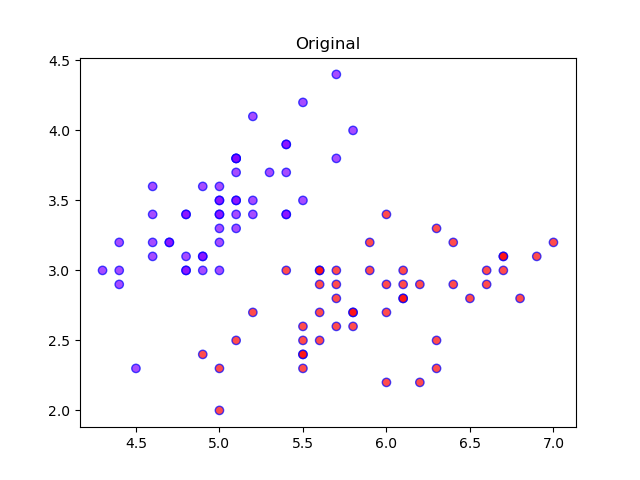
\includegraphics[width=4.96in,height=3.73in]{./media/image38.png}
	\end{Center}
\end{figure}


%%%%%%%%%%%%%%%%%%%% Figure/Image No: 28 Ends here %%%%%%%%%%%%%%%%%%%%

\par

\textcolor[HTML]{202122}{Training/Fitting}\par



%%%%%%%%%%%%%%%%%%%% Figure/Image No: 29 starts here %%%%%%%%%%%%%%%%%%%%

\begin{figure}[H]
	\begin{Center}
		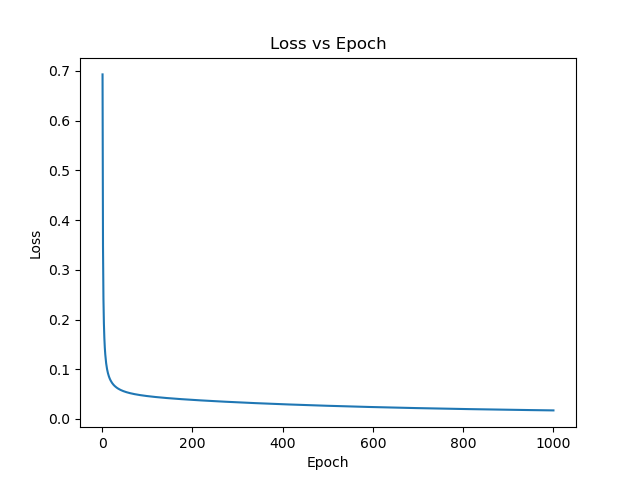
\includegraphics[width=5.46in,height=4.1in]{./media/image39.png}
	\end{Center}
\end{figure}


%%%%%%%%%%%%%%%%%%%% Figure/Image No: 29 Ends here %%%%%%%%%%%%%%%%%%%%

\par

\textcolor[HTML]{202122}{Output Predictions}\par



%%%%%%%%%%%%%%%%%%%% Figure/Image No: 30 starts here %%%%%%%%%%%%%%%%%%%%

\begin{figure}[H]
	\begin{Center}
		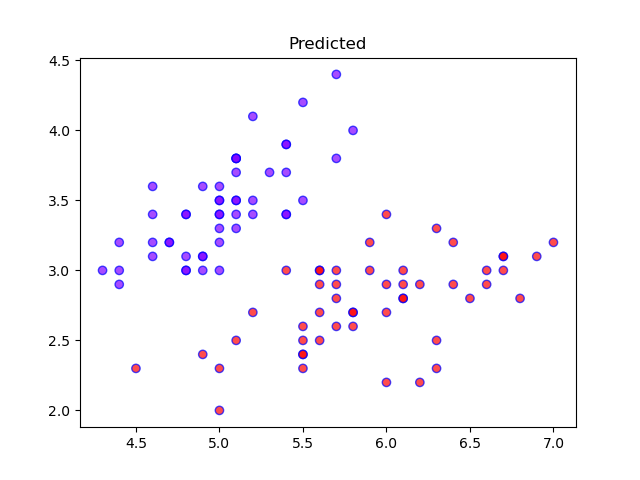
\includegraphics[width=5.48in,height=4.12in]{./media/image40.png}
	\end{Center}
\end{figure}


%%%%%%%%%%%%%%%%%%%% Figure/Image No: 30 Ends here %%%%%%%%%%%%%%%%%%%%

\par


\printbibliography
\end{document}